\documentclass[journal,12pt,onecolumn,draftclsnofoot]{IEEEtran}
\IEEEoverridecommandlockouts
% The preceding line is only needed to identify funding in the first footnote. If that is unneeded, please comment it out.
\def\BibTeX{{\rm B\kern-.05em{\sc i\kern-.025em b}\kern-.08em
    T\kern-.1667em\lower.7ex\hbox{E}\kern-.125emX}}


%\usepackage{movie15} % gif
\usepackage{comment}
\usepackage{cite}
\usepackage{amsmath,amssymb,amsfonts}
\usepackage{graphicx}
\usepackage{textcomp}
\usepackage{xcolor}
\usepackage{todonotes}
\usepackage{subcaption}
\captionsetup{compatibility=false}
\usepackage{caption}
%\usepackage{algorithm}
\usepackage[noend]{algorithmic}
\usepackage{url}
%\usepackage{titlesec}
\usepackage{authblk}
\usepackage{blindtext}
\usepackage[switch]{lineno}

\usepackage{booktabs}

\usepackage{multirow}
\usepackage{makecell}

\usepackage[switch]{lineno}

\usepackage{color, colortbl}

%\usepackage{algorithmicx}
%\usepackage{algpseudocode}
\usepackage[linesnumbered, ruled]{algorithm2e}
\SetKwRepeat{Do}{do}{while}%

\renewcommand{\linenumberfont}{\normalfont\tiny\color{red}}

%!TEX root = matmul_wse.tex


\newcommand{\wse}{{{WSE-2}}\xspace}
\newcommand{\gemm}{{{GEMM}}\xspace}
\newcommand{\matmul}{{\texttt{MatMul}}\xspace}
\newcommand{\master}{{\texttt{MASTER}}\xspace}
\newcommand{\summa}{{\texttt{SUMMA}}\xspace}
\newcommand{\async}{{\texttt{Async\_execution}}\xspace}

\looseness=1
\widowpenalty=500

\begin{document}
%\linenumbers

% Title
\title{General Matrix Multiply on CS-2}

\author[1,2]{Qinglei Cao}

\affil[1]{Cerebras Systems, US}
\affil[2]{\textit {\{qinglei.cao\}@cerebras.net}}

\maketitle

%\begin{abstract}
%\input{abstract.tex}
%\end{abstract}

%\begin{IEEEkeywords}
%\end{IEEEkeywords}

%%%%%%%%%%%%%%%%%%%%%%%%%%%%%%%%%%%%%%%%%%%%%%%%%%%%%%%%%%%%%%%%%%%%%%%%%%
\section{The Cerebras CS-2}
\label{sec:intro}
%!TEX root = matmul_wse.tex


\begin{figure}[b!]
  \centering
  \begin{subfigure}{0.70\columnwidth}
    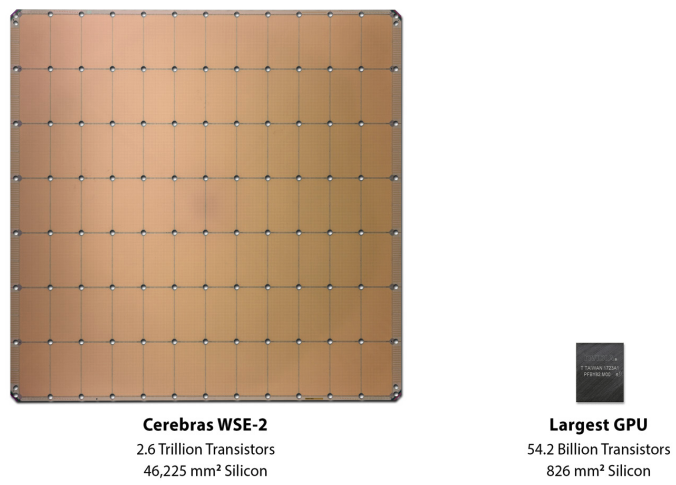
\includegraphics[width=\linewidth]{figures/wse2_vs_gpu.png}
  \end{subfigure}
  \caption{The Cerebras WSE-2 and the largest Graphics Processing Unit in comparison.}
  \label{fig:wse2_vs_gpu}
\end{figure}

The CS-2 is a system solution that consists of innovations across three dimensions: a) the second generation Cerebras Wafer Scale Engine (\wse) — the industry’s largest and only multi-trilliontransistor processor, b) the Cerebras System and c) the Cerebras software platform.
%
\wse is the processor at the heart of the CS-2, which is the largest chip ever built, as demonstrated in Figure~\ref{fig:wse2_vs_gpu}.
%
It is the industry’s only multi-trillion transistor processor, and contains more cores, more local memory, and more fabric bandwidth than any chip in history.
%
This enables fast, flexible computation at lower latency and with less energy.

The \wse covers 46,255 square millimeters — 56 times larger than the largest graphics processing unit.
With 850,000 cores, 40 Gigabytes of on-chip SRAM, 20 petabytes/sec of memory bandwidth, and 220
petabits/sec of interconnect bandwidth, the WSE-2 contains 123 times more compute cores, 1,000 times
more high-speed on-chip memory, 12,862 times more memory bandwidth and 45,833 times more fabric
bandwidth than its graphics processing competitor. In effect, it provides the compute capacity of an entire
cluster in a single chip, without the cost, complexity, and bandwidth bottlenecks involved with lashing
together hundreds of smaller devices. A summary of the comparison is shown in Figure~\ref{fig:wse2_vs_a100}.

\begin{figure}[t!]
  \centering
  \begin{subfigure}{0.90\columnwidth}
    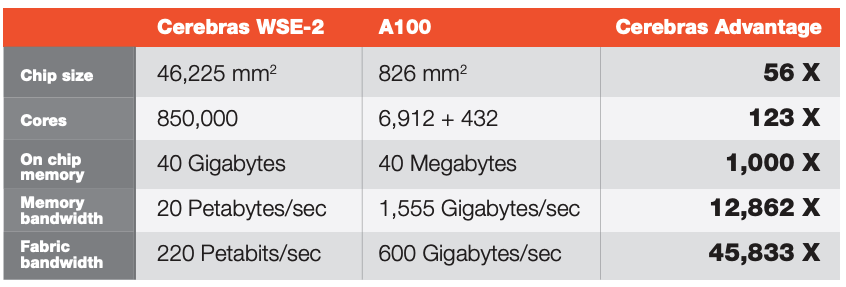
\includegraphics[width=\linewidth]{figures/wse2_vs_a100.png}
  \end{subfigure}
  \caption{Overview of the magnitude of advancement made by the Cerebras WSE-2}
  \label{fig:wse2_vs_a100}
\end{figure}



\begin{figure}[b!]
  \centering
  \begin{subfigure}{0.90\columnwidth}
    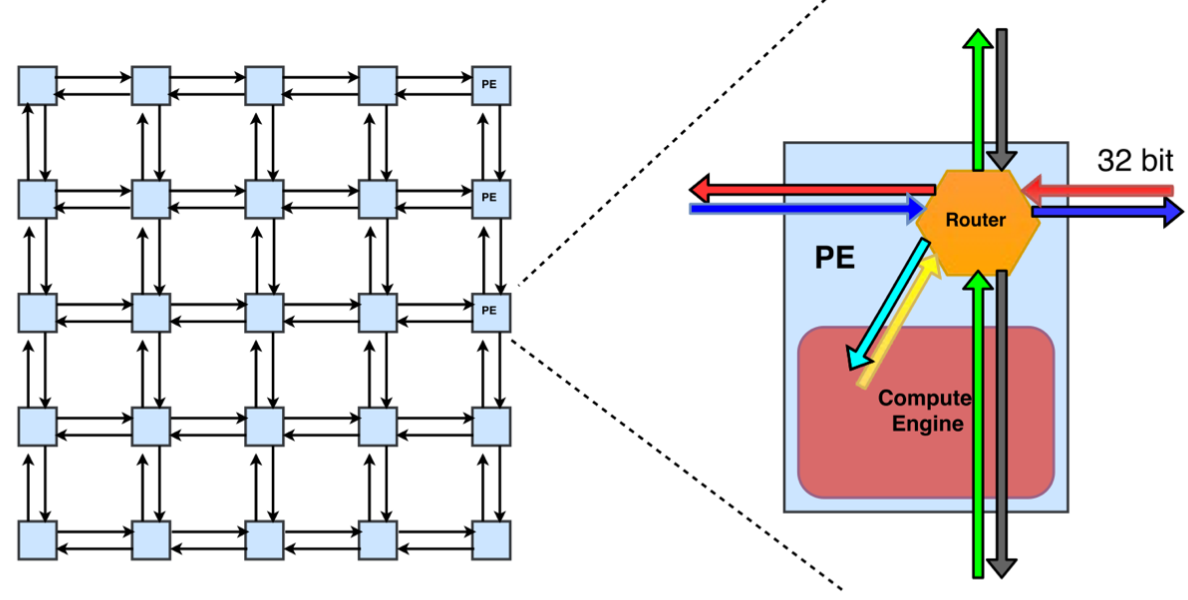
\includegraphics[width=\linewidth]{figures/pe.png}
  \end{subfigure}
  \caption{\wse organizations}
  \label{fig:pe}
\end{figure}



More details, the Cerebras Swarm communication fabric creates a massive on-chip network that delivers breakthrough bandwidth and low latency, at a fraction of the power draw of traditional communication techniques that are used to aggregate servers of graphics processing units into large clusters.
%
Swarm connects all 850,000 cores on the Cerebras \wse in a 2D-mesh with 220 Petabits/sec of
bandwidth (Figure~\ref{fig:pe} left).
%
Swarm provides a hardware routing engine to each of the cores and connects them with short wires optimized for bandwidth and low-latency. 
%
The resulting fabric supports single-word active messages that can be received by the cores without any software overhead, providing flexible, allhardware communication.
%
%
Each core is called processing element (PE), which is consist of a fabric router and a compute engine (CE), as shown in Figure~\ref{fig:pe} (right).


The router is a 5-port switch, with 1 port for each of the cardinal directions (North, South, East, and West), and one port for the CE.
%
The fabric router supports 24 virtual channels, called colors.
%
The switching unit is a wavelet, which consists of 32 data bits, one control bit, and 5 color bits. 
%
Wavelets are separated into two categories: control wavelets and data wavelets.
%
The fabric can receive a single wavelet per cycle from each of the 5 router ports and can send one wavelet per cycle on each of the 5 router ports.
%
The connection from fabric to compute engine is referred to as the “offramp”, and the connection from CE to fabric is called the "onramp".
%
Sitting at the boundary between the CE and the fabric are a set of queues and filters:
%
\begin{itemize}
  \item four filters, which can be used to selectively discard wavelets on the offramp;
  \item eight input queues, each of which is associated with a fabric color and serves as an extension of the fabric queue from the perspective of the CE;
  \item six output queues, holding wavelets generated by the CE until the fabric can accept them.
\end{itemize}


A CE is a simple compute core that runs instructions from memory.
%
Tasks are the primary unit of programming with only one task executing at a time.
%
There are two broad categories of tasks: wavelet-triggered tasks (WTTs) and local tasks. 
%
The scheduler can only choose to run tasks that are both unblocked and activated.
\begin{itemize}
  \item Wavelet-triggered tasks are activated by the arrival of wavelets, whether it be data wavelets or control 
  wavelets.
  %
  Data wavelets activate the data task associated with their color, while control wavelets activate the control tasks associated with the entry-point they store in bits 0 to 5 of the index field.
  \item Local tasks, on the other hand, can be activated by microthreads on completion or by FIFOs on pop or push.
  %
  They can also be activated using the {\it actvt} instruction.
\end{itemize}
%
Instructions that operate on vectors, which are described using data-structure registers (DSRs), are one of the important hardware features.
%
There are three main modes of execution: normal mode, single-step mode, and microthread mode.
\begin{itemize}
  \item In normal mode, vector instructions run until they complete.
  \item Single-step mode is similar to normal, but vector operands can be looped over so operations that require multiple instructions per-element can be executed.
  \item Microthread mode is quite different different and is a method of processing vectors that are received or transmitted on the fabric in a manner which does not require the processor to stall waiting for inputs or outputs to become available.
  %
  A microthreaded instruction is launched as part of a normal task, which then executes until it runs out of resources.
  %
  If it is unable to complete execution, it then effectively forks itself off to become an independent single-instruction task. 
  %
  Microthreads can be run concurrently with other tasks.
\end{itemize}

\begin{figure}[b!]
  \centering
  \begin{subfigure}{0.70\columnwidth}
    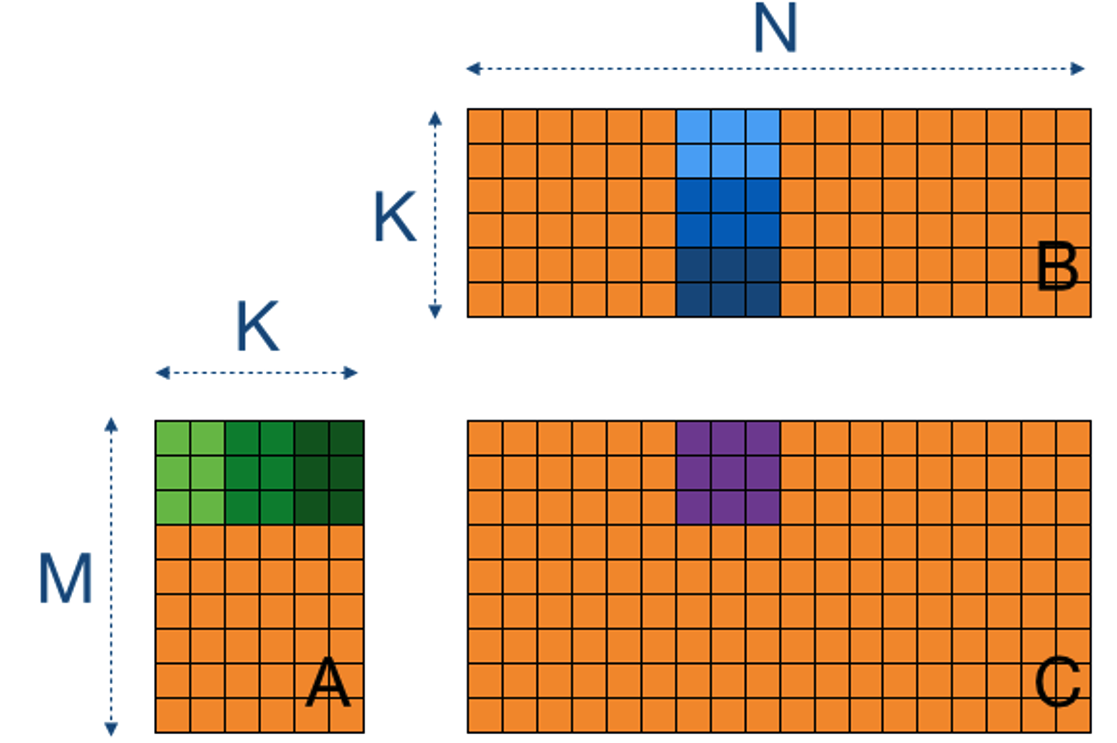
\includegraphics[width=\linewidth]{figures/gemm_overview.png}
  \end{subfigure}
  \caption{GEMM example}
  \label{fig:gemm_overview}
\end{figure}

Memory is a key component of every computer architecture. 
%
Memory closer to compute translates to faster calculation, lower latency, and better power efficiency for data movement. 
%
The \wse has 40 Gigabytes of on-chip memory, all uniformly distributed alongside the cores, and 20 Petabytes/sec of memory bandwidth, i.e., each PE holds 48KB on-chip memory and reads/writes at the rate of 32 bits/cycle.
%%%%%%%%%%%%%%%%%%%%%%%%%%%%%%%%%%%%%%%%%%%%%%%%%%%%%%%%%%%%%%%%%%%%%%%%%%
\section{General Matrix Multiply}
\label{sec:gemm}
%!TEX root = matmul_wse.tex

\begin{figure}[b!]
  \centering
  \begin{subfigure}{0.40\columnwidth}
    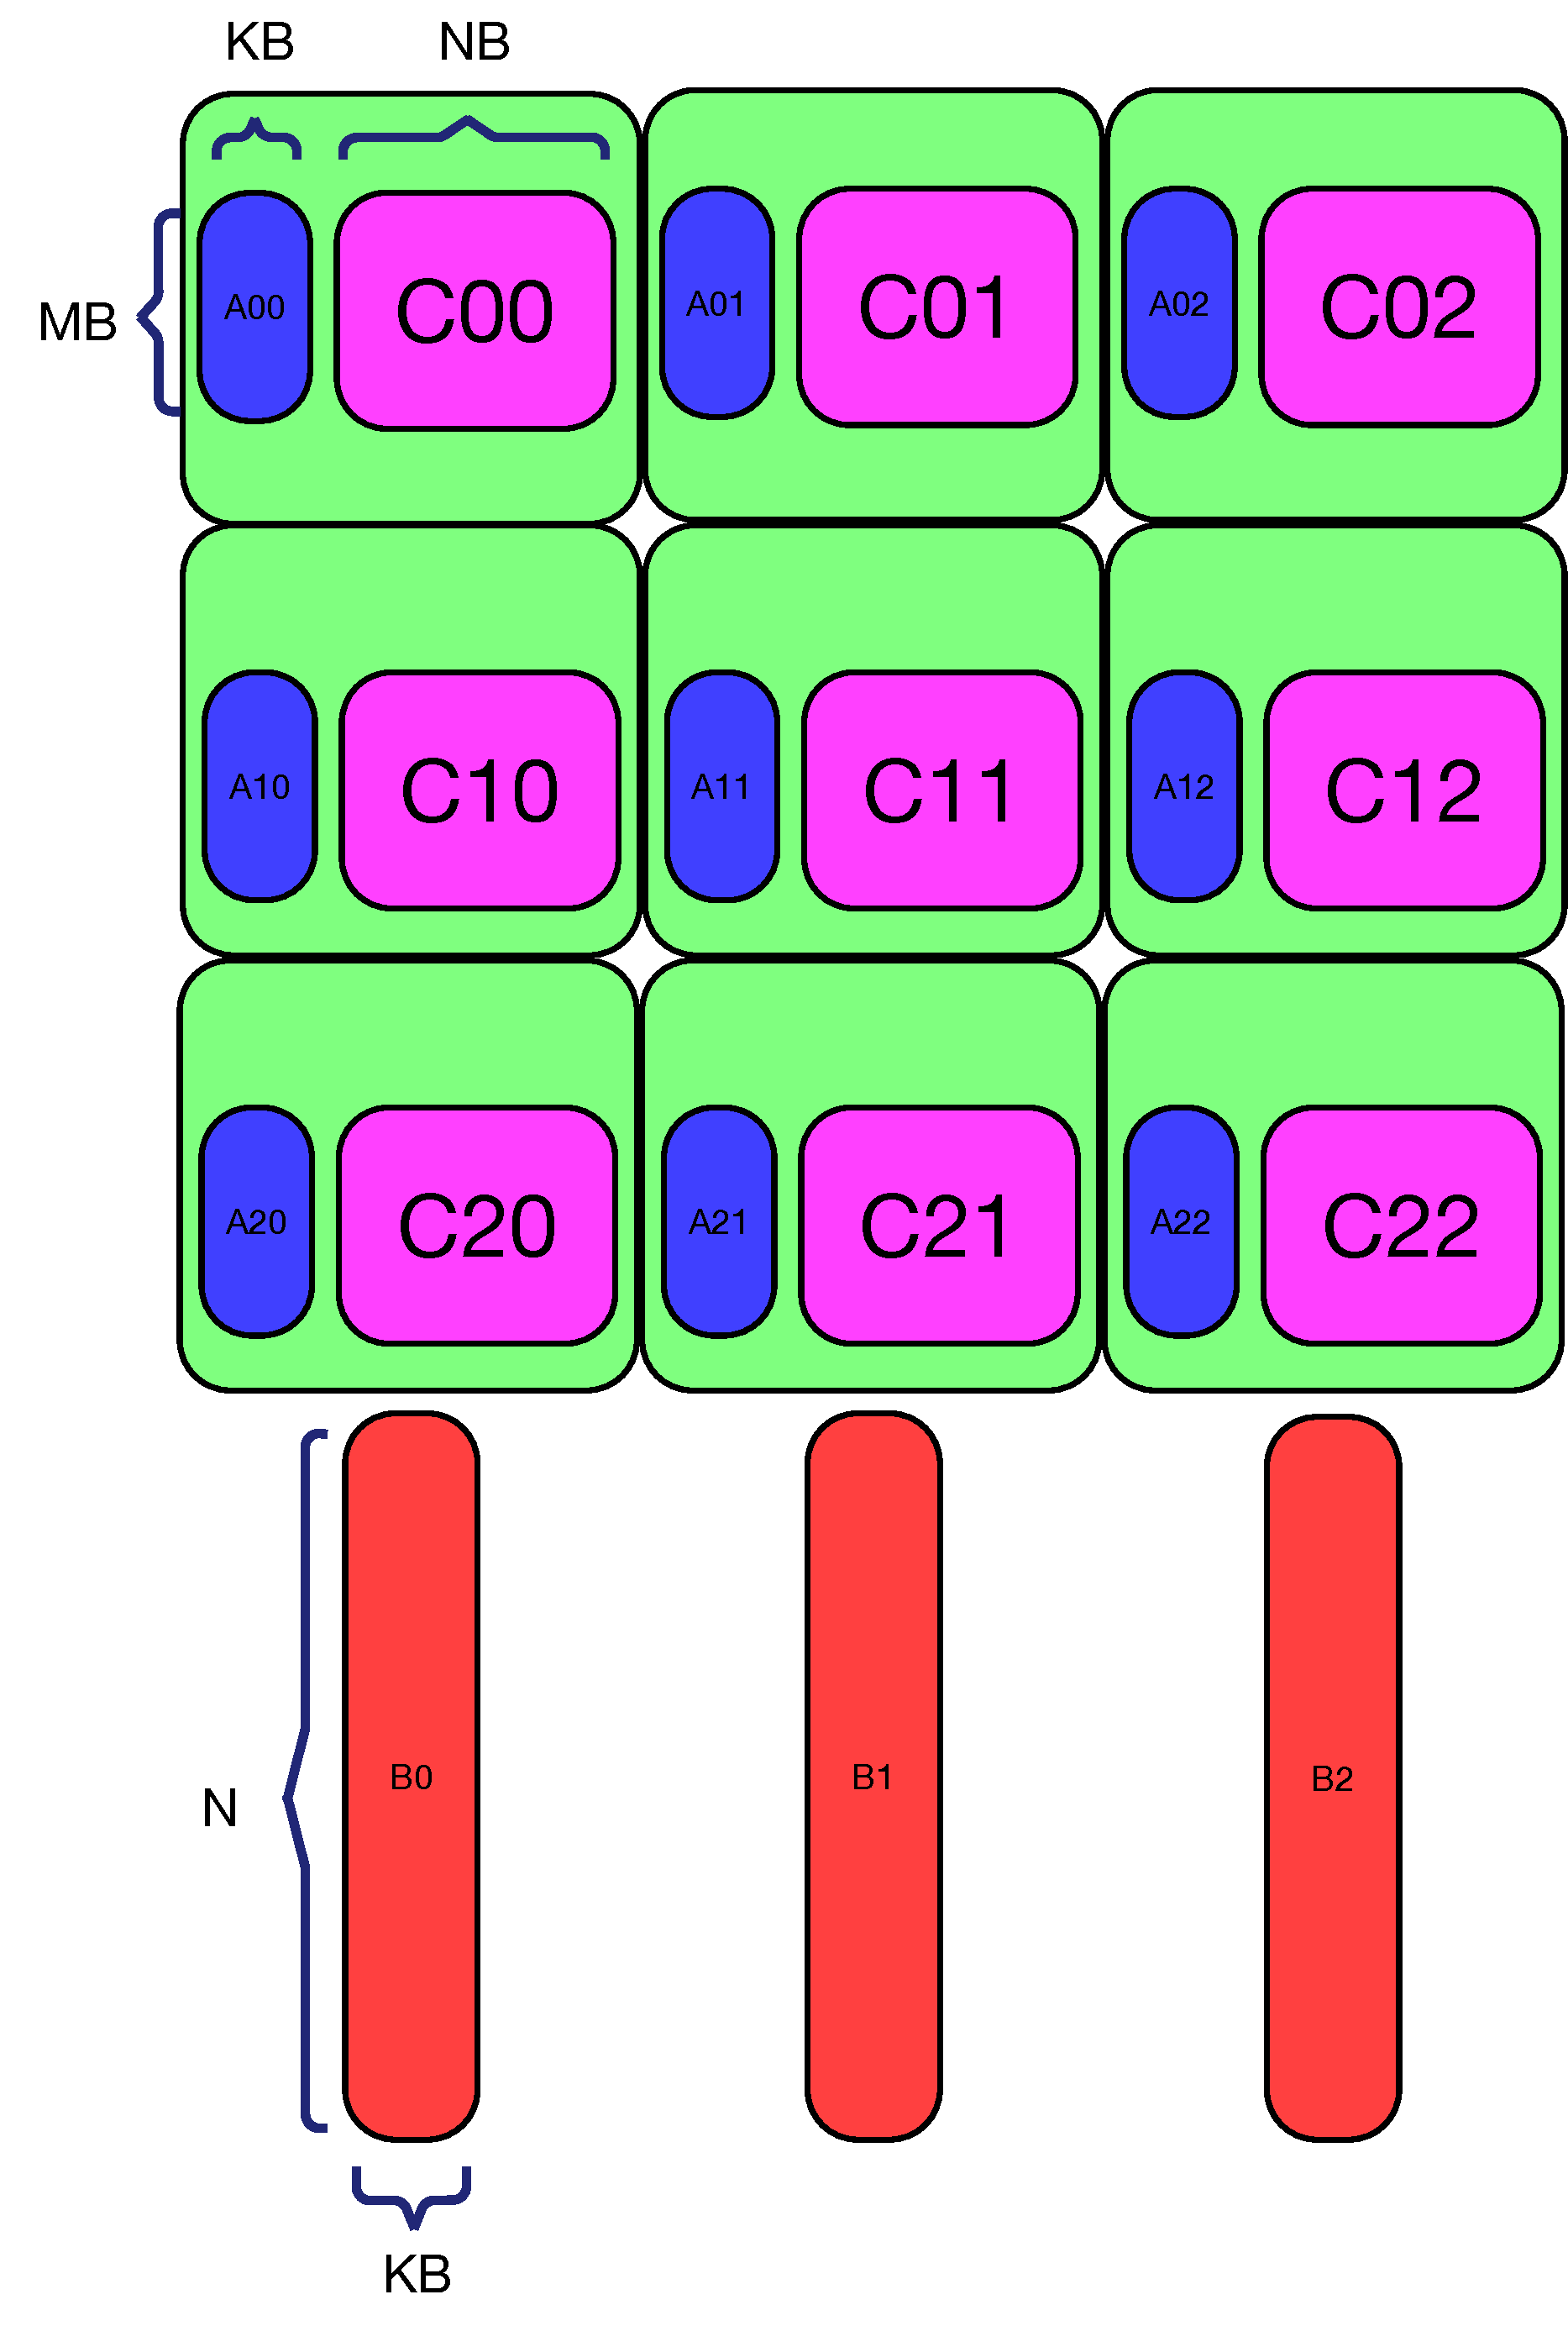
\includegraphics[width=\linewidth]{figures/gemm_A_C_memory_master/1.pdf}
    \caption{Data distribution.}
    \label{fig:gemm_master_1}
  \end{subfigure}
  %
  \begin{subfigure}{0.40\columnwidth}
    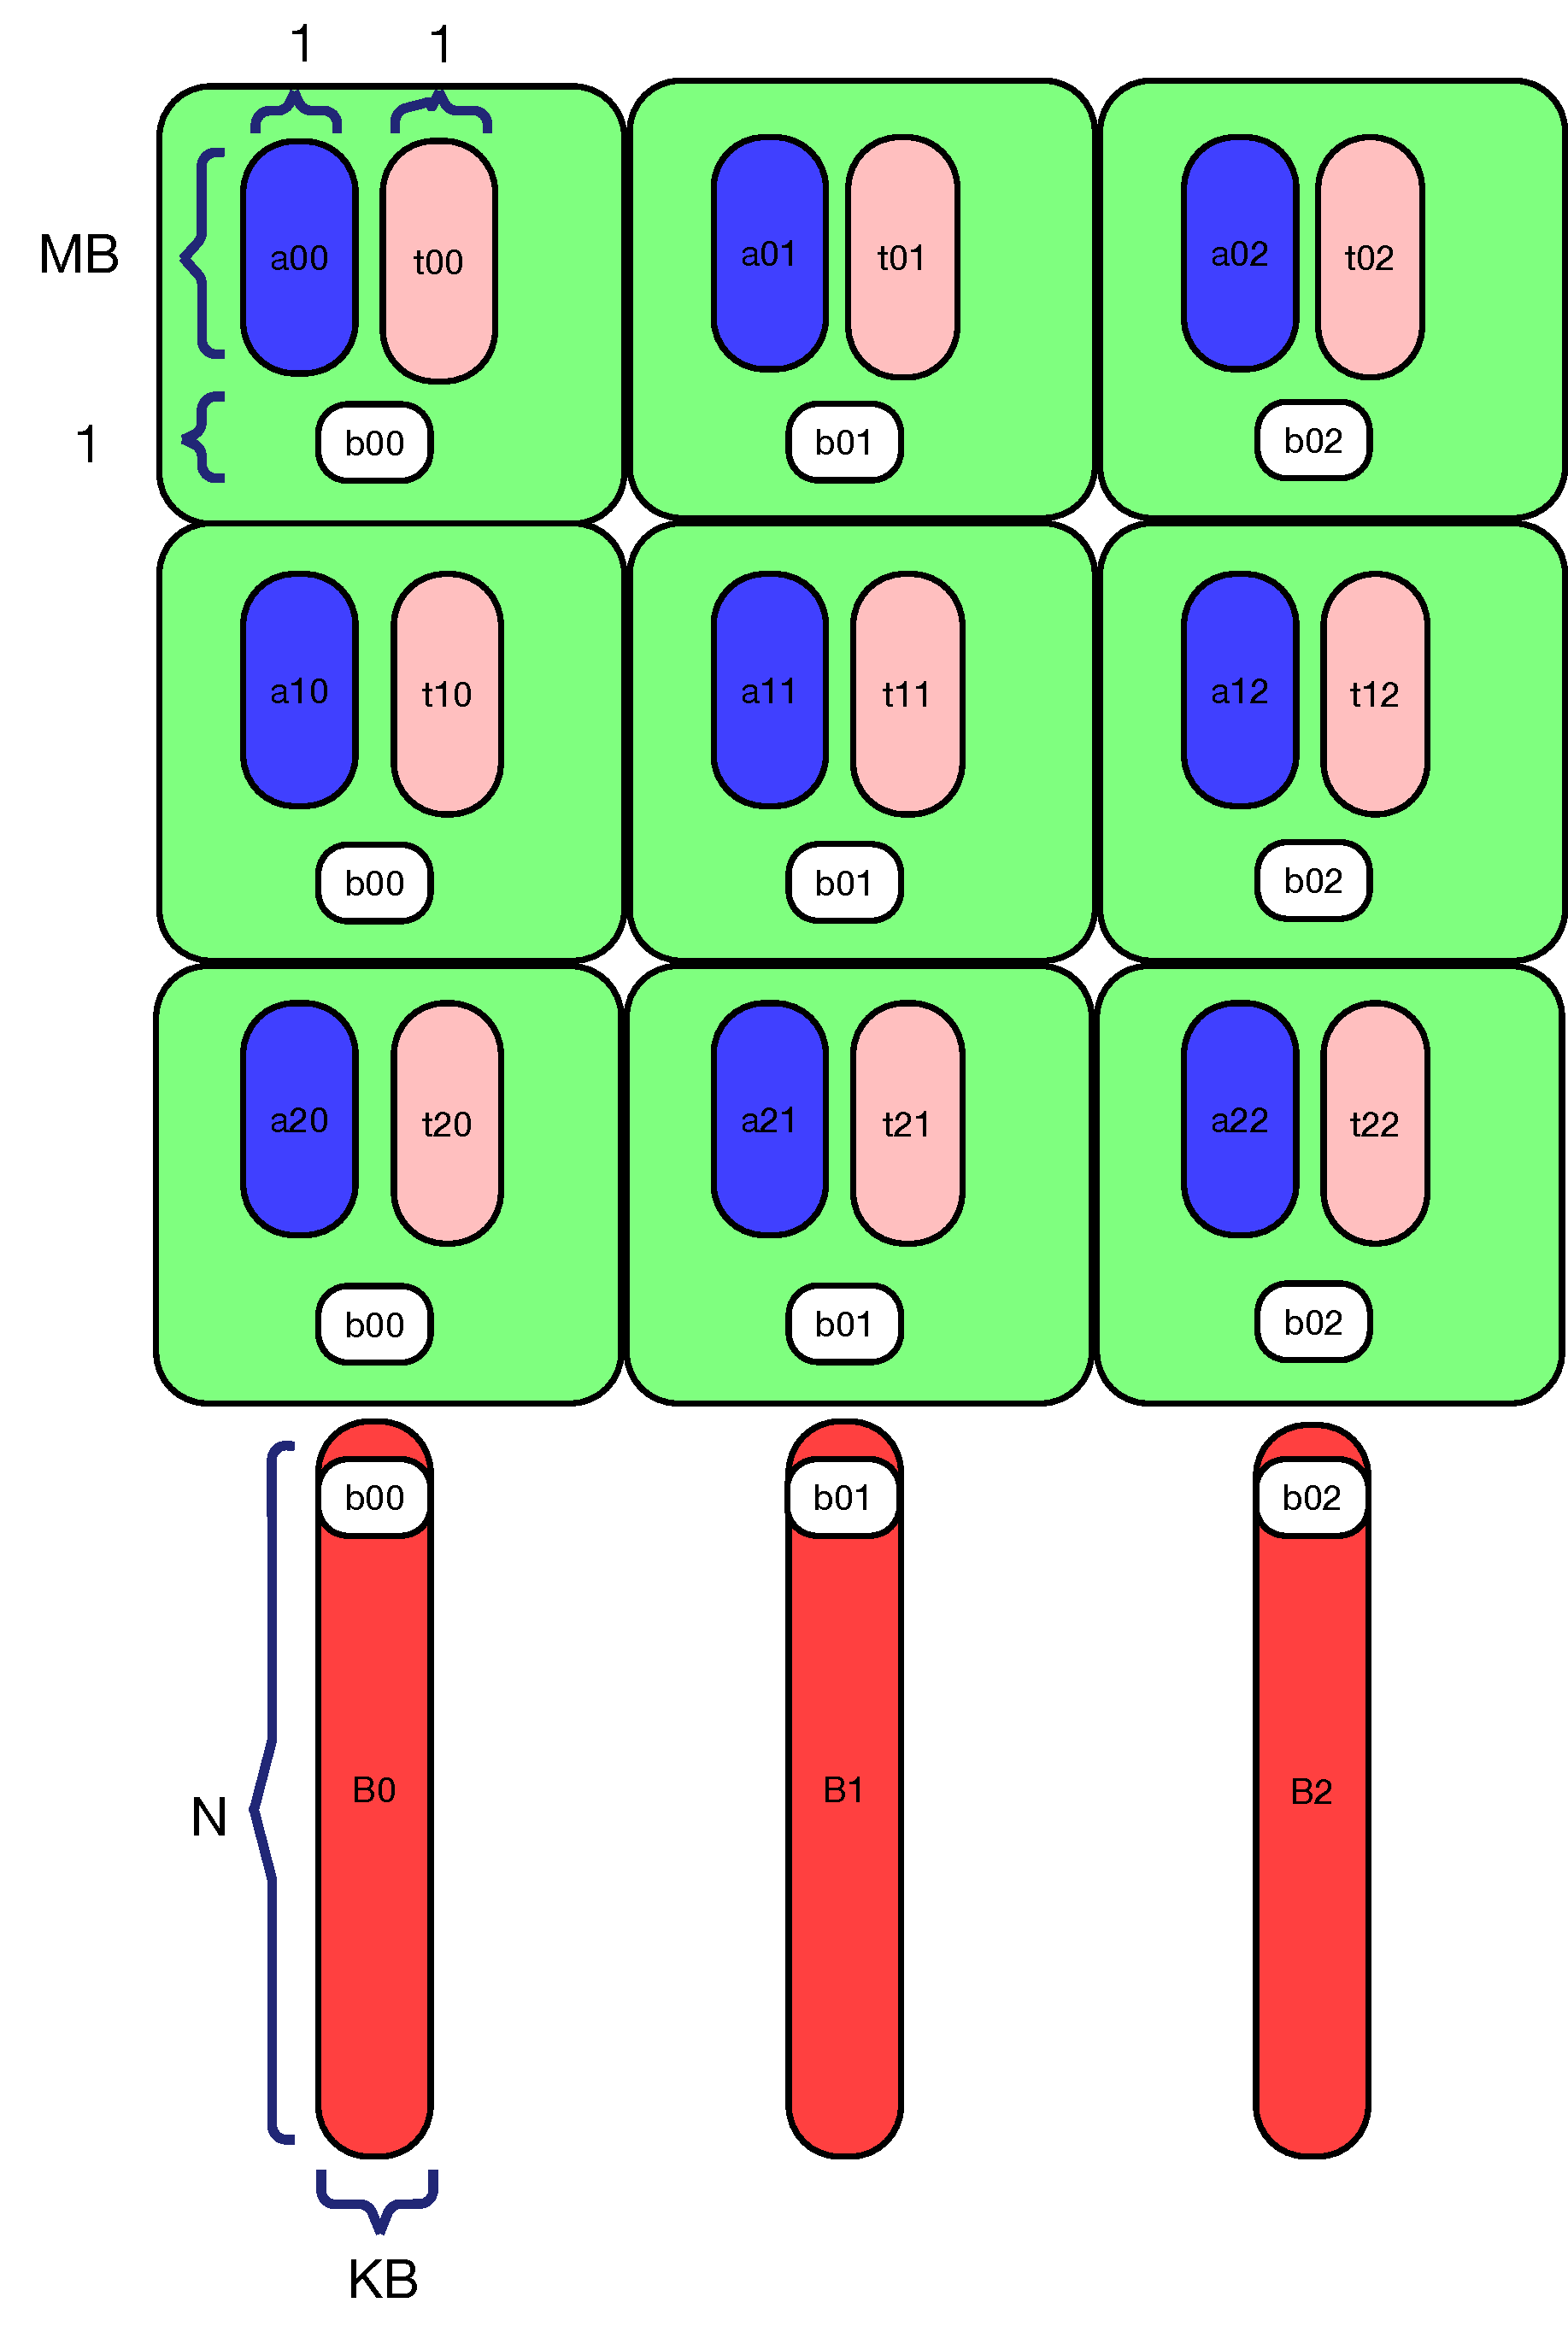
\includegraphics[width=\linewidth]{figures/gemm_A_C_memory_master/2.pdf}
    \caption{The first iteration.}
    \label{fig:gemm_master_2}
  \end{subfigure}
  \caption{\master.}
  \label{fig:gemm_master}
\end{figure}

General Matrix Multiply (\gemm) is a common but widely-used algorithm in linear algebra, machine learning, statistics, and many other domains.
%
It is a level-3 routine in Blas Linear Algebra Subprograms (BLAS)~\cite{blas}, which is compute intensive with $O(N^3)$ flops and $O(N^2)$ data movement, where N is the matrix size.
%
Figure~\ref{fig:gemm_overview} demonstrates an example of ${C}_{M \times N} = A_{M \times K} B_{K \times N}$.
%
Here, a special scenario is considered, called \matmul kernel in weight streaming (WS).
%
It is a variant of \gemm, where one of the inputs ($A$ and $B$) is streamed in from fabric (one feature for \wse).
%
Without loss of generality, let $B$ be streamed in from fabric as weight and $A$ and $C$ be stored in memory as activation, to remove the transpose in the real implementation.
%
Two algorithms are compared, i.e., the method used in the current master (called \master hereinafter) and Scalable Universal Matrix Multiplication Algorithm (\summa~\cite{van1997summa}).
%%%%%%%%%%%%%%%%%%%%%%%%%%%%%%%%%%%%%%%%%%%%%%%%%%%%%%%%%%%%%%%%%%%%%%%%%%
\section{\master}
\label{sec:master}
%!TEX root = matmul_wse.tex

\subsection{Implementation}


Figure~\ref{fig:gemm_master_1} depicts how the data is distributed across PEs in \master, where $A$ and $C$ are distributed on $3 \times 3$ PEs ($PE_x = PE_y = 3$), $PE_x \times KB = K$, $PE_x \times NB = N$, and $PE_y \times MB = M$.
%
The way what \master does is to calculate the final result in $C$ one column by one column.
%
Take the calculation of the first column in $C$ for instance, as shown in Figure~\ref{fig:gemm_master_2}.
%
One column in $B$ is streamed in so that each PE receives a vector of size $KB$.
%
Then, $MB \times KB$ number of FMAC instructions (floating multiply-add) are operated locally, which output results to temporary buffers, holding the partial of the final results.
%
Therefore, a row reduction is required to generate the final result of the first column in $C$, as shown in Figure~\ref{fig:gemm_master_3} which reduces $t0*$, $t*$ and $t2*$ to the corresponding target $C$ column sequentially.


\begin{figure}[t!]
  \centering
  \begin{subfigure}{0.70\columnwidth}
    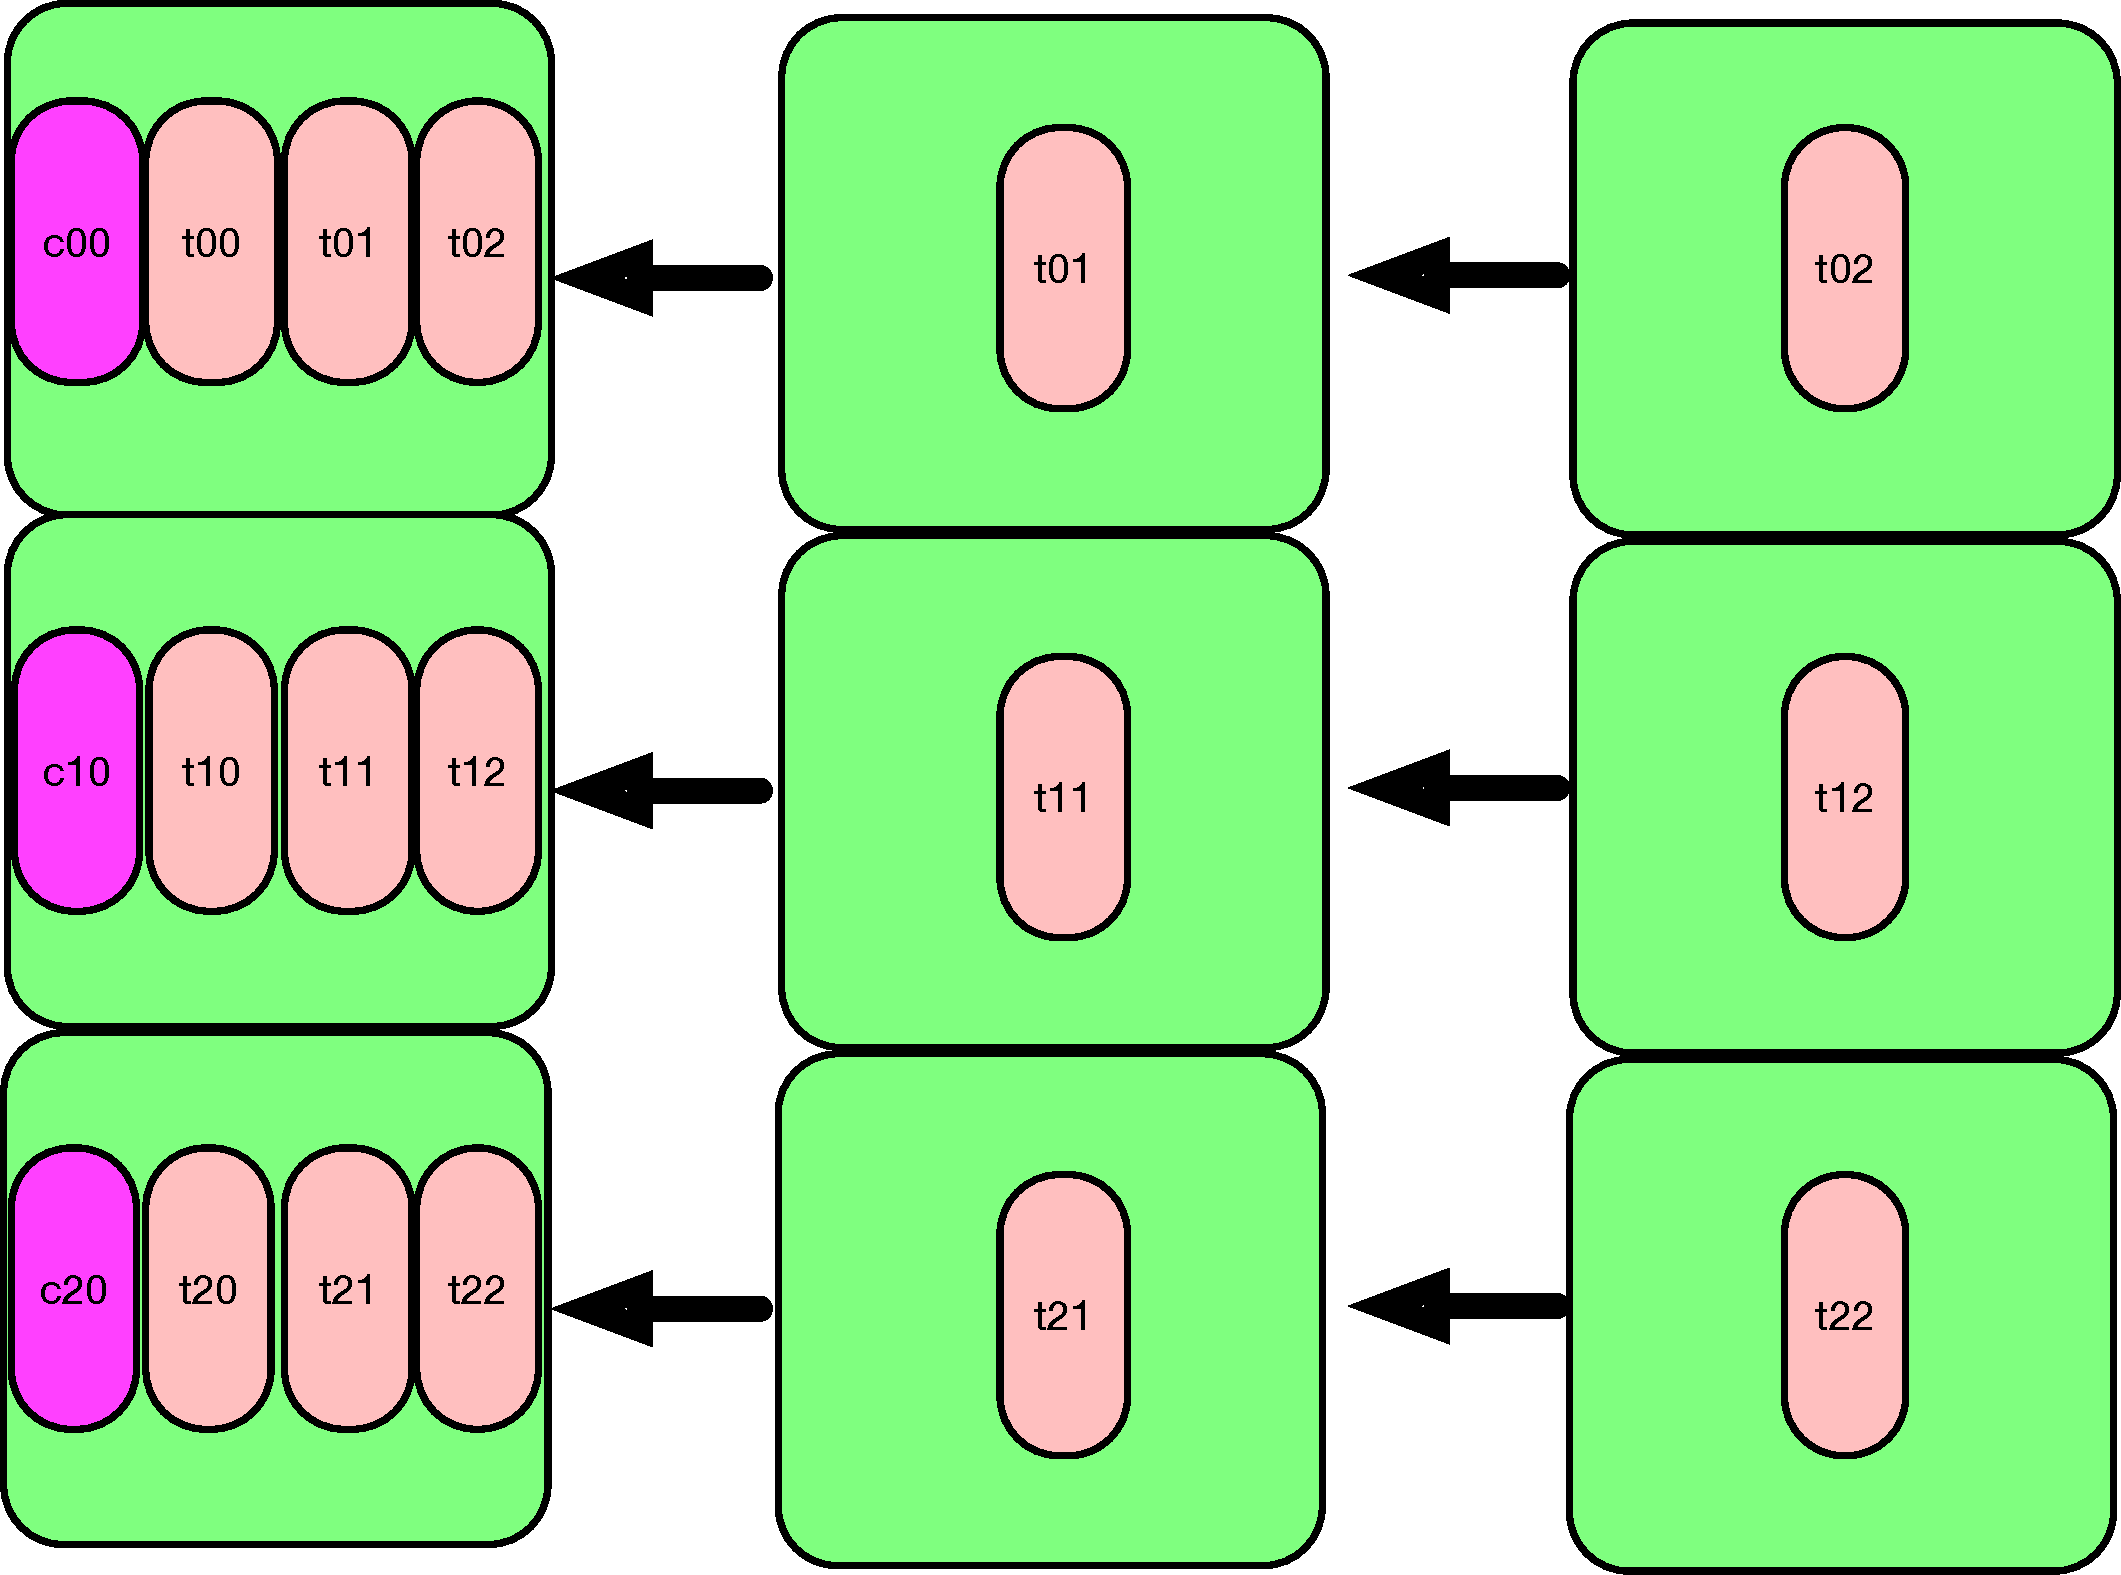
\includegraphics[width=\linewidth]{figures/gemm_A_C_memory_master/3.pdf}
  \end{subfigure}
  \caption{Row reduction, reducing from the temporary buffer to the target column in $C$}
  \label{fig:gemm_master_3}
\end{figure}

\subsection{Performance Analysis}

\begin{figure}[t!]
  \centering
  \begin{subfigure}{0.48\columnwidth}
    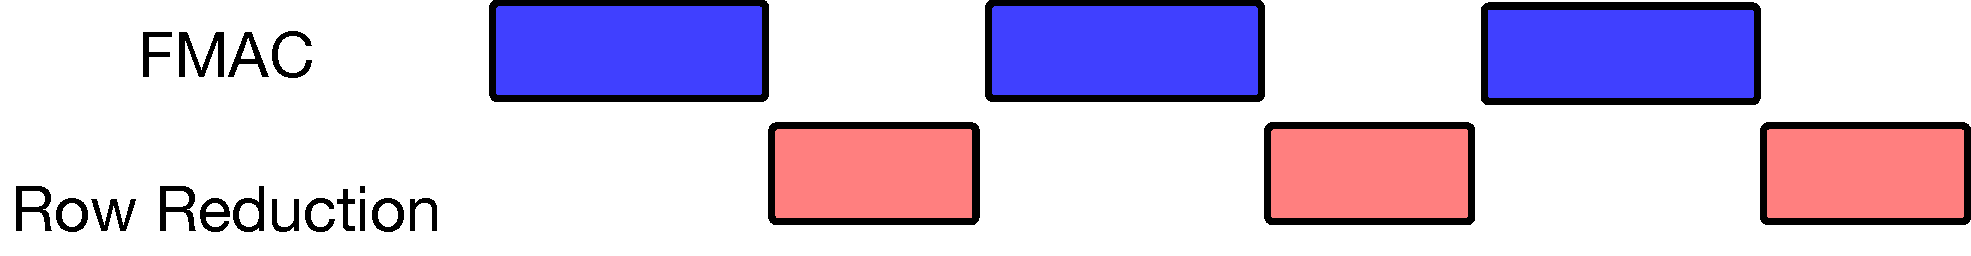
\includegraphics[width=\linewidth]{figures/gemm_A_C_memory_master/4.pdf}
    \caption{Mathematical}
  \end{subfigure}
  \hfill
  \begin{subfigure}{0.48\columnwidth}
    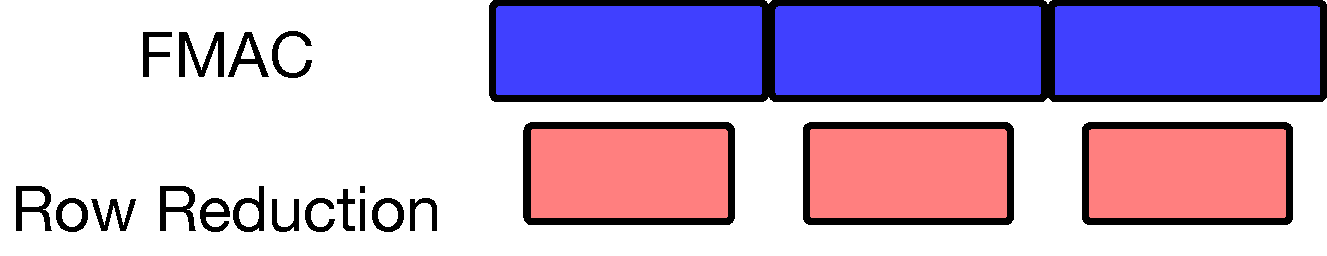
\includegraphics[width=\linewidth]{figures/gemm_A_C_memory_master/41.pdf}
    \caption{Optimal}
  \end{subfigure}
  \caption{Execution of \master}
  \label{fig:gemm_master_4}
\end{figure}


\begin{figure}[t!]
  \centering
  \begin{subfigure}{0.40\columnwidth}
    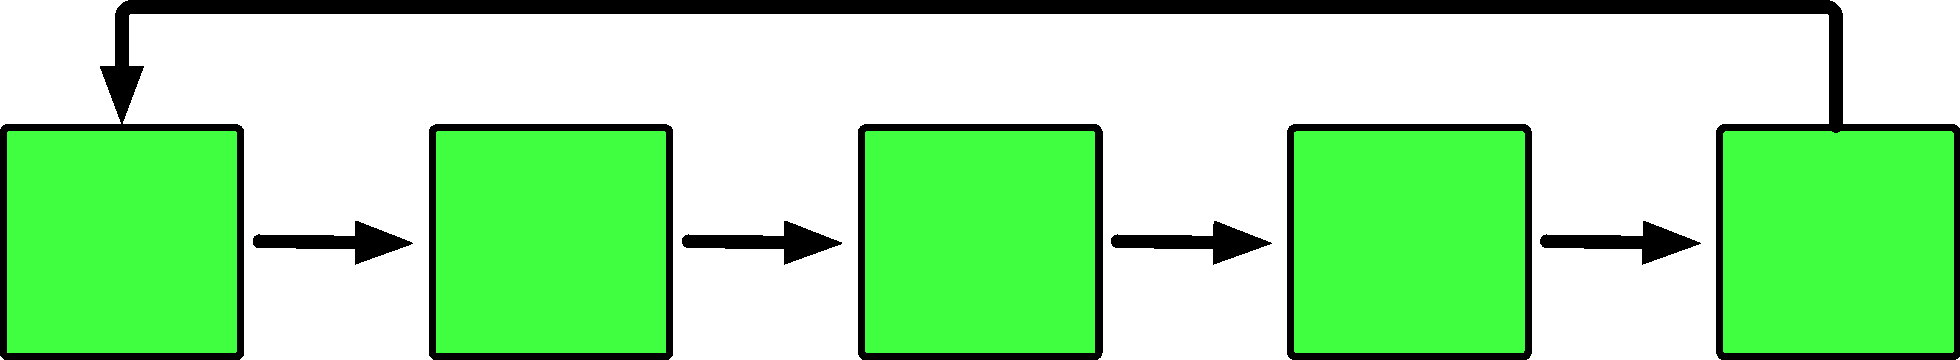
\includegraphics[width=\linewidth]{figures/gemm_A_C_memory_master/5.pdf}
    \caption{Flat ring.}
    %\label{fig:gemm_master_1}
  \end{subfigure}
  \hfill
  %
  \begin{subfigure}{0.40\columnwidth}
    
\includegraphics[width=\linewidth]{figures/gemm_A_C_memory_master/6.pdf}
    \caption{Jump ring.}
    %\label{fig:gemm_master_2}
  \end{subfigure}
  \caption{Communication pattern.}
  \label{fig:gemm_master_5_6}
\end{figure}


The execution model of \master can be described in Figure~\ref{fig:gemm_master_4}.
%
From mathematical perspective, $MB \times KB$ number of FMAC instructions are followed by a row reduction along horizontal split across vertical split.
%
However, in practice, many optimizations have been proposed to approach its optimal which overlaps FMACs and row reductions, including asynchronous execution (\async) and double buffering.
%
From the section above, it can be seen that each iteration, i.e., calculation of each column in $C$, is independent, as well as each row of PEs.
%
Therefore, if only considering one iteration of the one PE which operates $FMAC$, the number of FMAC is $nb\_fmac = MB \times KB$, followed by $nb\_fsum = MB \times PE_x$ number of reduction (FSUM, floating sum).
%
Take \async for instance, whose purpose is to hide the overhead of row reduction by FMAC.
%
This \async has two aspects: (1) executing FMACs and FSUMs asynchronously (2) executing FSUMs of different PEs asynchronously.
%
Therefore, if the communication pattern in row reduction is jump ring (see Figure~\ref{fig:gemm_master_5_6}) and the data is operated in half-precision, i.e., FP16 (SIMD = 4),
\begin{itemize}
  \item the number of cycles of FMAC: $cycle\_fmac = nb\_fmac/4$
  \item the number of cycles of FSUM: $cycle\_fsum = 1 + 3 \times PE_x + MB/4$ (2 cycles to send data to its dependent and 1 cycle of FSUM, pipelined)
\end{itemize}
%
Hence, if discarding the potential overlap of FSUM between iterations, the efficiency it can achieve in theory is $\frac{cycle\_fma}{max(cycle\_fmac, cycle\_fsum) + MB/4}$, i.e., 
\begin{equation}
  efficiency = \frac{MB \times KB}{max(MB \times KB, 4 + 12 \times PE_x) + MB}
  \label{eq:master}
\end{equation}
%
(Data movement can be dealt by microthread asynchronously, while FMAC and FSUM are operated by main thread.)

If FSUMs between iterations are perfectly overlapped, then theoretical efficiency is:
\begin{equation}
  efficiency = \frac{MB \times KB \times N}{(MB \times KB + MB) \times N + 12 \times PE_x}
  \label{eq:master_2}
\end{equation}
%
%In other words,
%\begin{itemize}
%%  \item if $MB \times (KB-1) \geq 12 \times PE_x$, it is: $KB/(KB+1)$;
%  \item if $MB \times (KB-1) < 12 \times PE_x$, it is: $MB \times KB/(MB \times KB+MB+12 \times PE_x) < 50\%$
%\end{itemize}
%
%Therefore, the condition above is critical 
%




%\includegraphics{summa_gemm.gif}

%%%%%%%%%%%%%%%%%%%%%%%%%%%%%%%%%%%%%%%%%%%%%%%%%%%%%%%%%%%%%%%%%%%%%%%%%%
\section{\summa}
\label{sec:summa}
%!TEX root = matmul_wse.tex

\subsection{Implementation}


\begin{figure}[t!]
  \centering
  \begin{subfigure}{0.40\columnwidth}
    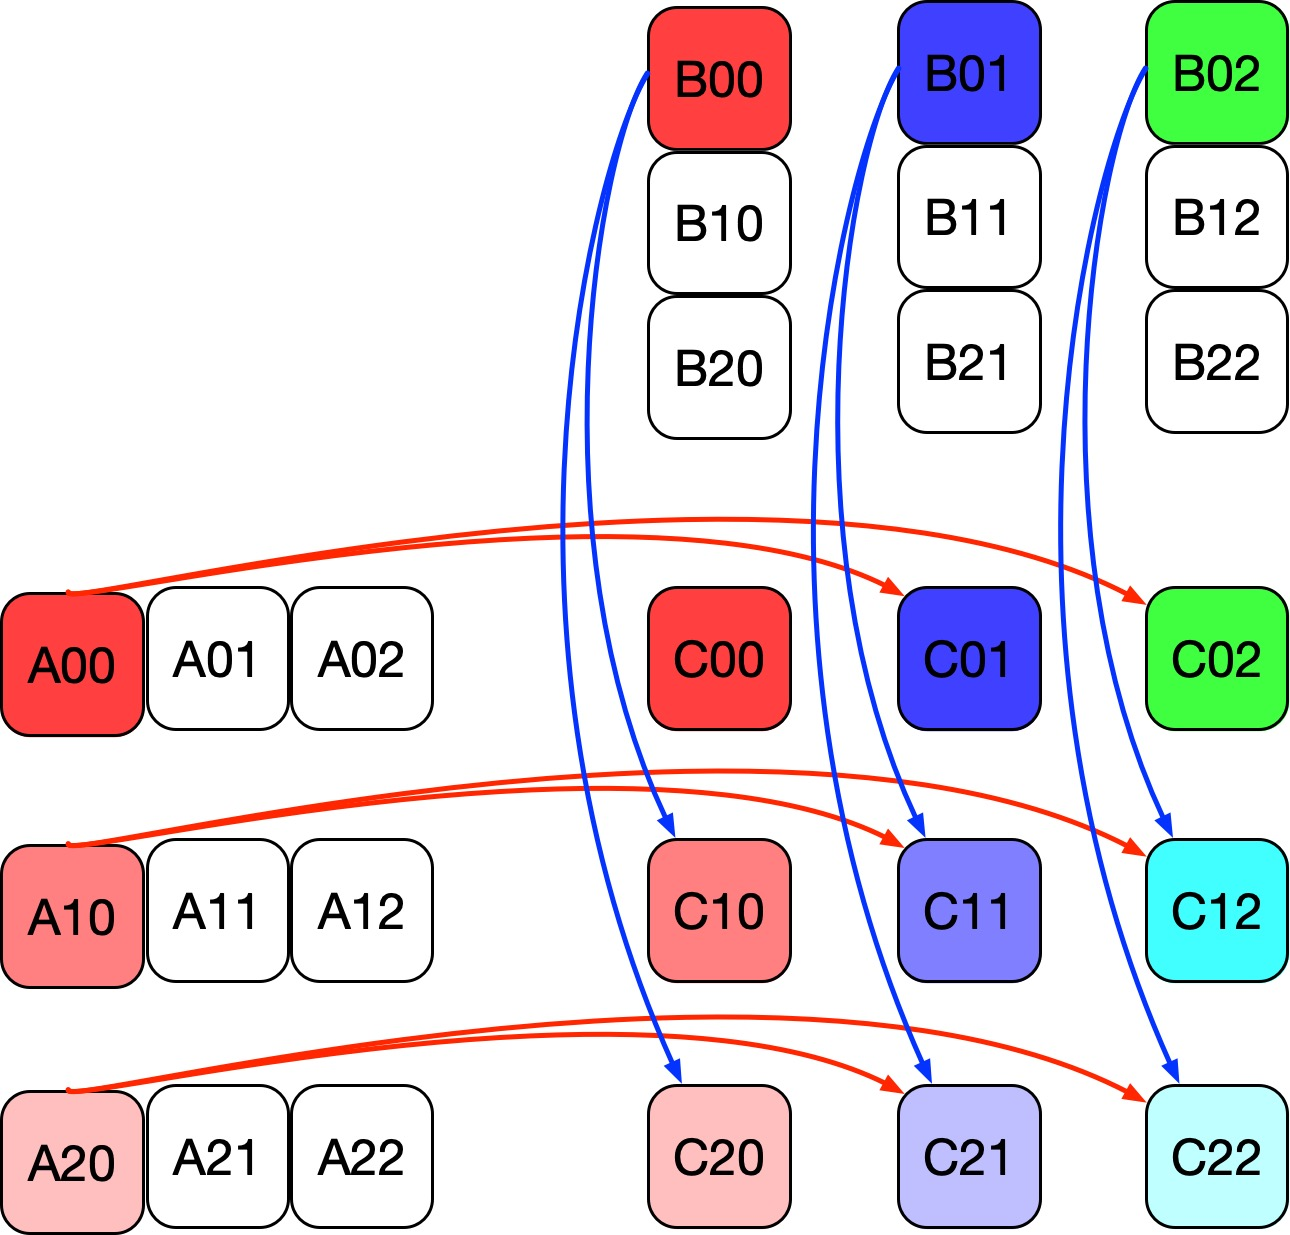
\includegraphics[width=\linewidth]{figures/gemm_summa_k0.jpg}
  \end{subfigure}
  \caption{Communication of \summa of the first iteration.}
  \label{fig:gemm_summa_k0}
\end{figure}



\begin{figure}[b!]
  \centering
  \begin{subfigure}{0.40\columnwidth}
    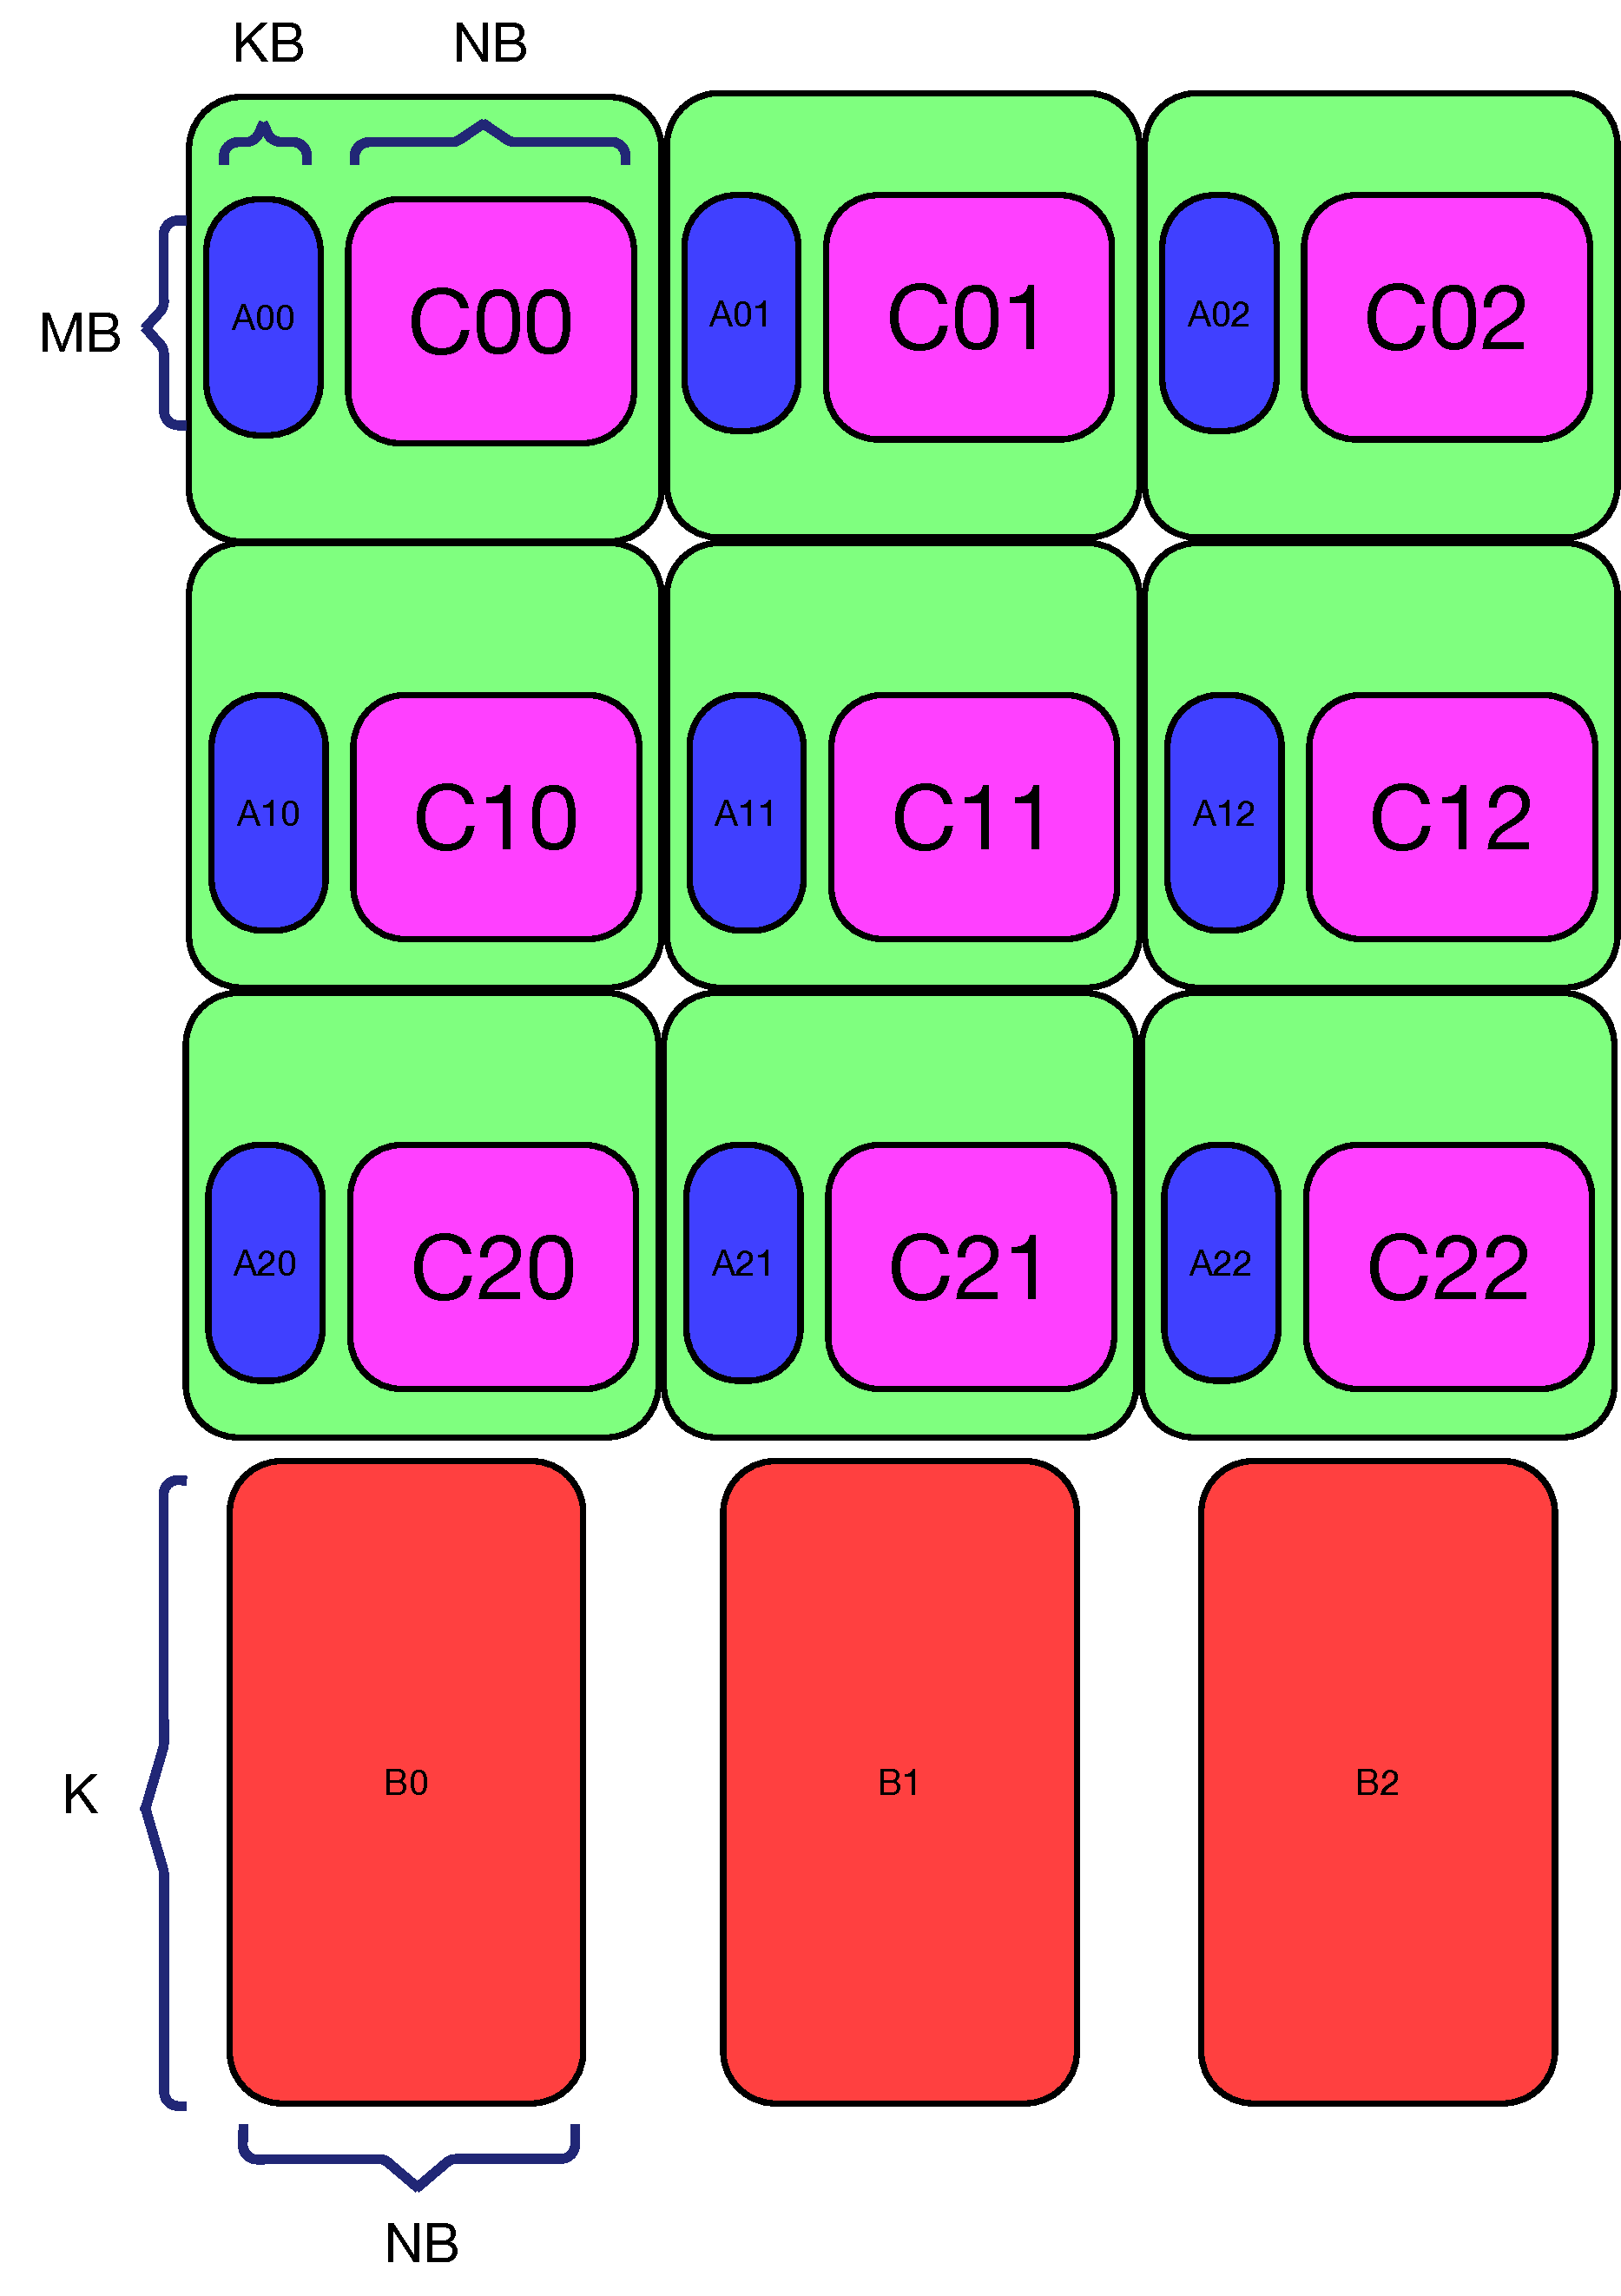
\includegraphics[width=\linewidth]{figures/gemm_A_C_memory_summa/1.pdf}
    \caption{Data distribution.}
    \label{fig:gemm_summa_1}
  \end{subfigure}
  \hfill
  %
  \begin{subfigure}{0.40\columnwidth}
    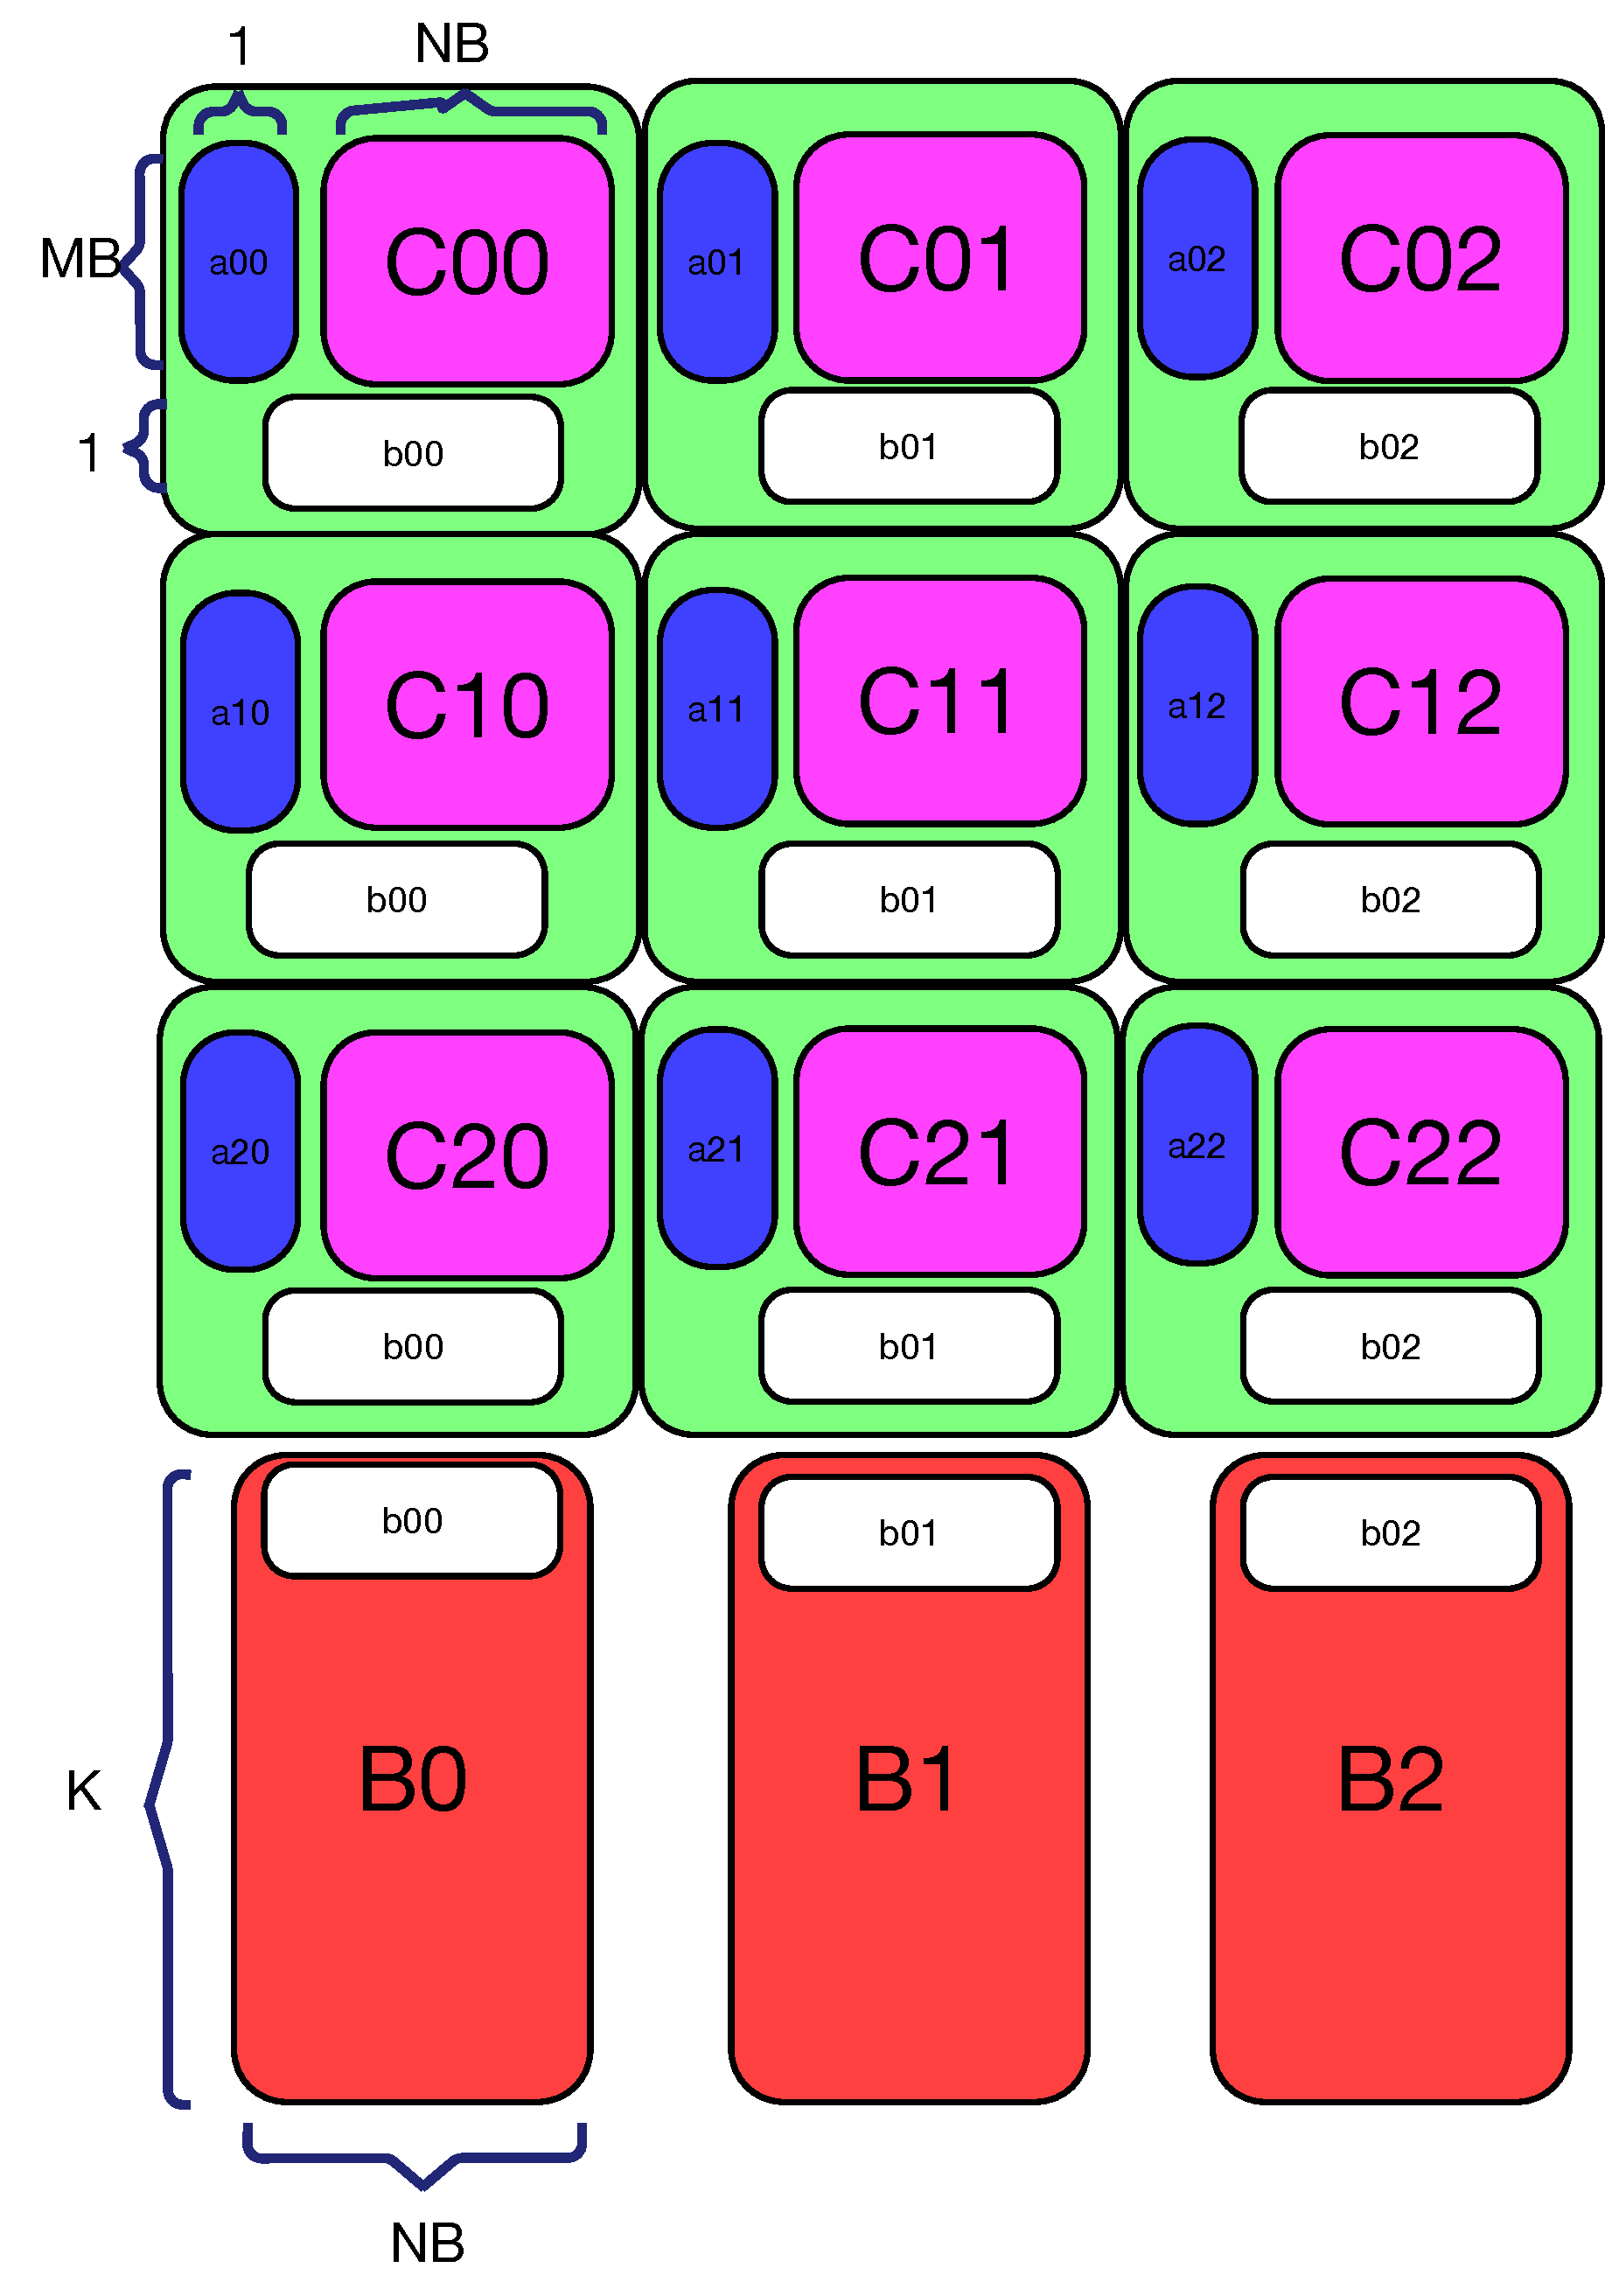
\includegraphics[width=\linewidth]{figures/gemm_A_C_memory_summa/2.pdf}
    \caption{The first iteration.}
    \label{fig:gemm_summa_2}
  \end{subfigure}
  \caption{\summa.}
  \label{fig:gemm_summa_1_2}
\end{figure}

\summa is one of the classical algorithms to solve matrix multiply problem~\cite{van1997summa}.
%
Figure~\ref{fig:gemm_summa_k0} shows the communication of the first iteration of \summa on $3 \times 3$ PEs/processes/blocks, which broadcasts $A$ horizontally, broadcasts $B$ vertically, and operates outer-produce between $A$ and $B$.
%
It can be seen that \summa consists of $K$ number of outer-product, and the vector sizes of each outer-product are $M$ and $N$.
%
Towards the special scenario where $B$ is streamed in, Figure~\ref{fig:gemm_summa_1} describes how the data is distributed, and Figure~\ref{fig:gemm_summa_2} shows the process of the first iteration, where $A$ and $C$ are distributed on $3 \times 3$ PEs ($PE_x = PE_y = 3$), $PE_x \times KB = K$, $PE_x \times NB = N$, and $PE_y \times MB = M$.


\subsection{Performance Analysis}


\begin{figure}[t!]
  \centering
  \begin{subfigure}{0.48\columnwidth}
    
\includegraphics[width=\linewidth]{figures/gemm_A_C_memory_summa/3.pdf}
    \caption{Mathematical}
  \end{subfigure}
  \hfill
  \begin{subfigure}{0.48\columnwidth}
    
\includegraphics[width=\linewidth]{figures/gemm_A_C_memory_summa/4.pdf}
    \caption{Optimal}
  \end{subfigure}
  \caption{Execution of \summa}
  \label{fig:gemm_summa_3_4}
\end{figure}


The execution model of \summa can be described in Figure~\ref{fig:gemm_summa_3_4} regarding its mathematical definition and the optimal goal.
%
As shown above, it can be seen: (1) each outer-product is independent; (2) the tile at the top right corner is the last to execute.
%
Therefore, if considering the first iteration of that PE in FP16, the number of FMAC is $nb\_fmac = MB \times NB$, using $nb\_fmac/4$ cycles.
%
For the communication overhead, that PE needs $PE_x + MB/2$ cycles (pipelined) to receive one piece of $A$ from West and $PE_y + NB/2$ cycles (pipelined) for the weight ($B$) from South.


First, let's see the efficiency that the mathematical definition can achieve.
%
If the two broadcasts of $A$ and $B$ can not be overlapped, then, the theoretically efficiency is 
\begin{equation}
  efficiency = MB \times NB/(MB \times NB+4 \times PE_x + 2 \times MB+4 \times PE_y + 2 \times NB)
  \label{eq:summa_1}
\end{equation}
%
If that two broadcasts can be overlapped, then
\begin{equation}
  efficiency= MB \times NB/(MB \times NB+max(4 \times PE_x + 2 \times MB, 4 \times PE_y + 2 \times NB))
  \label{eq:summa_2}
\end{equation}
%
Next, let's consider the optimal one, where FMAC and the two broadcasts can be overlapped, then
\begin{equation}
  efficiency = MB \times NB/max(MB \times NB, 4 \times PE_x + 2 \times MB, 4 \times PE_y + 2 \times NB)
  \label{eq:summa_3}
\end{equation}





%\includegraphics{summa_gemm.gif}

%%%%%%%%%%%%%%%%%%%%%%%%%%%%%%%%%%%%%%%%%%%%%%%%%%%%%%%%%%%%%%%%%%%%%%%%%%
\section{Experiments}
\label{sec:perf}
%!TEX root = matmul_wse.tex

%\subsection{Theoretical Simulation}
 
First, we simulate the theoretical performance \master and \summa based on the equations above, as shown in Figure~\ref{fig:gemm_perf_simulate} on three scenarios which varies $NB$ and $KB$ (10 and 70) but keeps $MB=70$.
%
We can see that, in theory, \master and \summa suits different scenarios while with the observation that on full scale wafer, (1)``MASTER\_OPT'' is better in the most cases; (2) ``SUMMA\_VECTOR\_OPT'' needs intensive computations to overlap the communication.

\begin{figure}[t!]
  \centering
  \begin{subfigure}{0.32\columnwidth}
    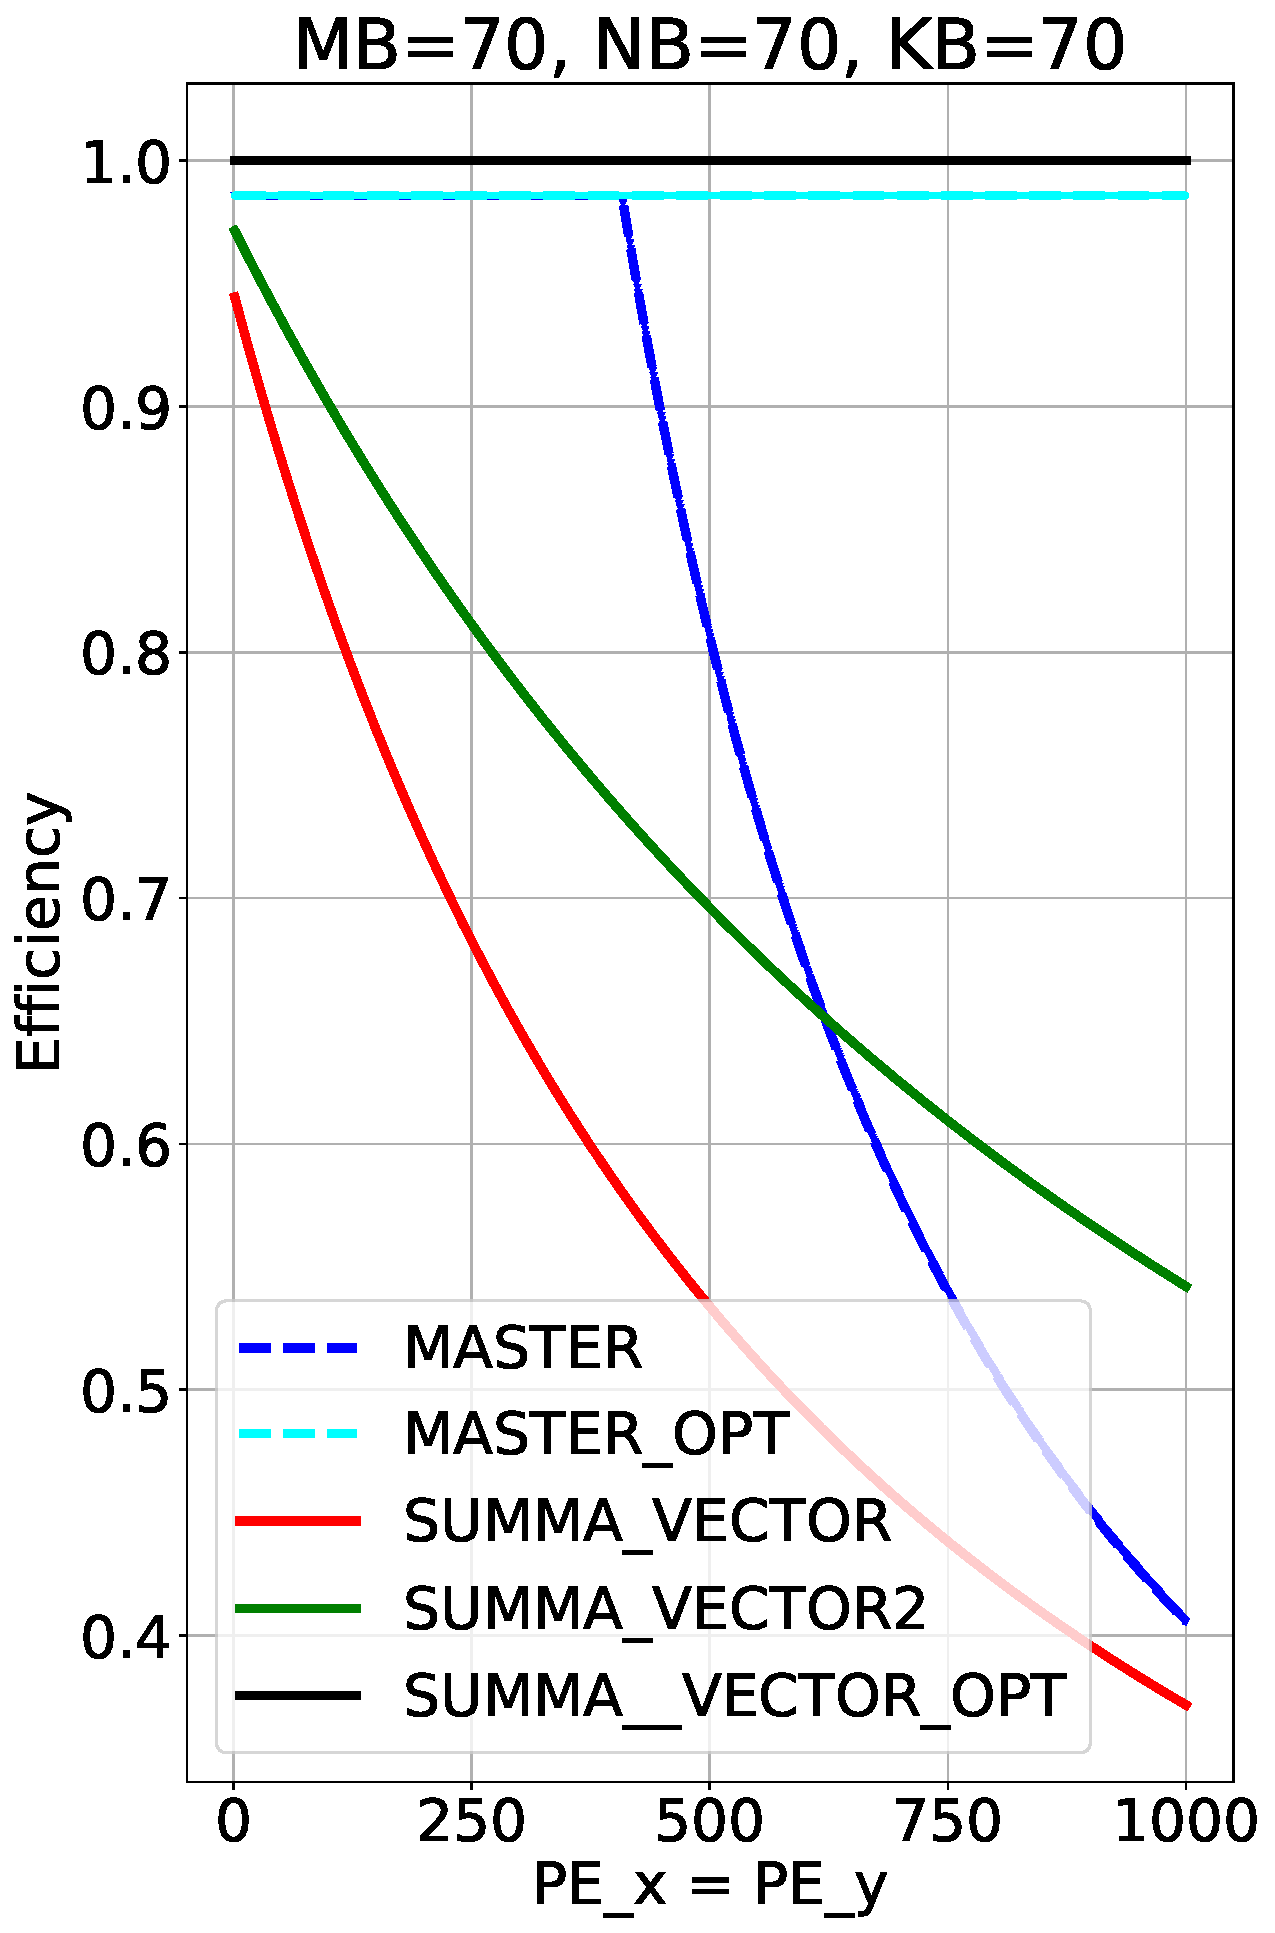
\includegraphics[width=\linewidth]{figures/efficiency_cost_70_70_70.pdf}
    %\caption{.}
    %\label{fig:gemm_master_1}
  \end{subfigure}
  \hfill
  %
  \begin{subfigure}{0.32\columnwidth}
    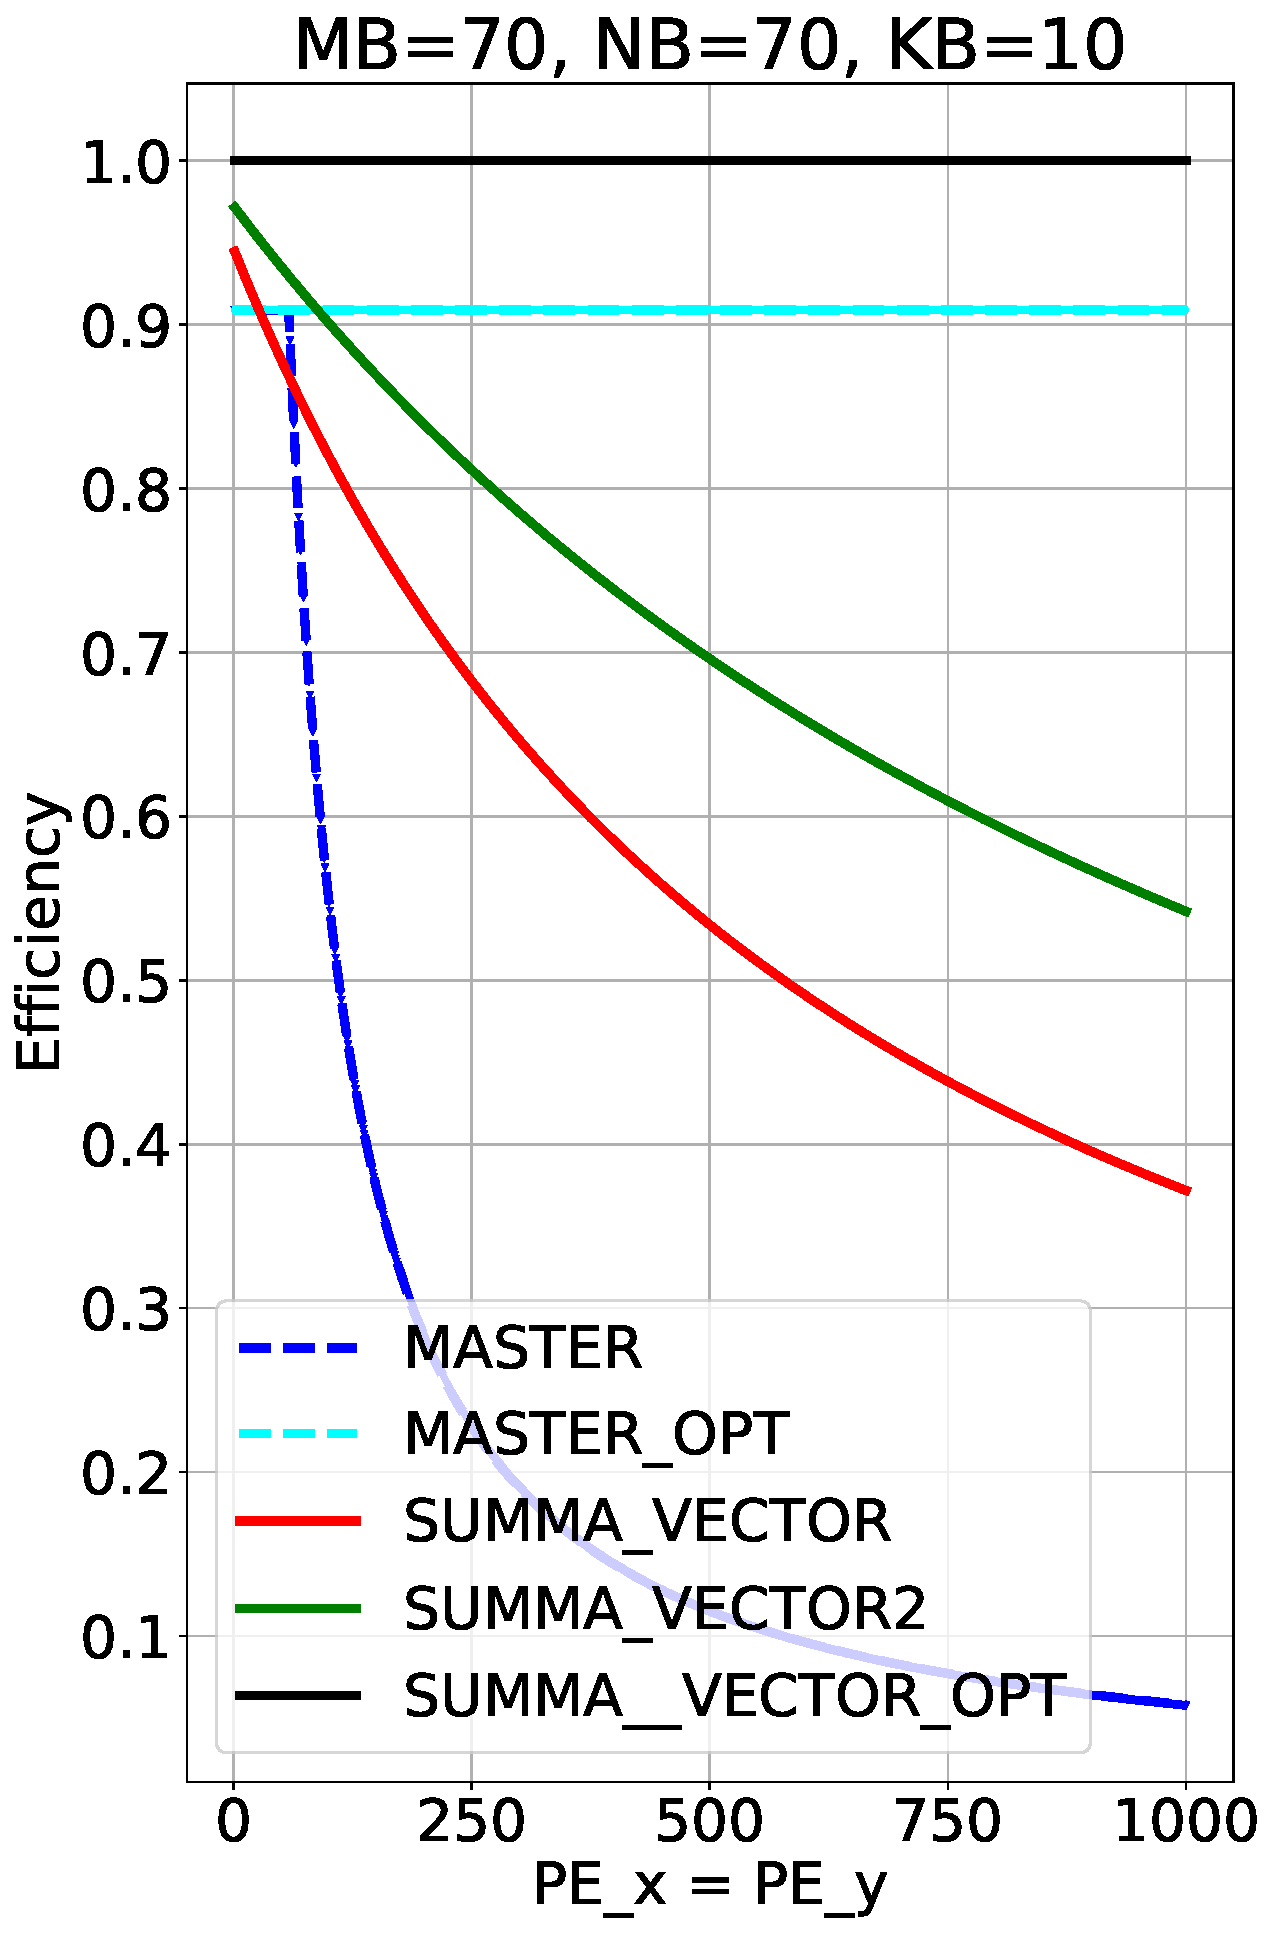
\includegraphics[width=\linewidth]{figures/efficiency_cost_70_70_10.pdf}
    %\caption{Non-ring.}
    %\label{fig:gemm_master_2}
  \end{subfigure}
  \hfill
  %
  \begin{subfigure}{0.32\columnwidth}
    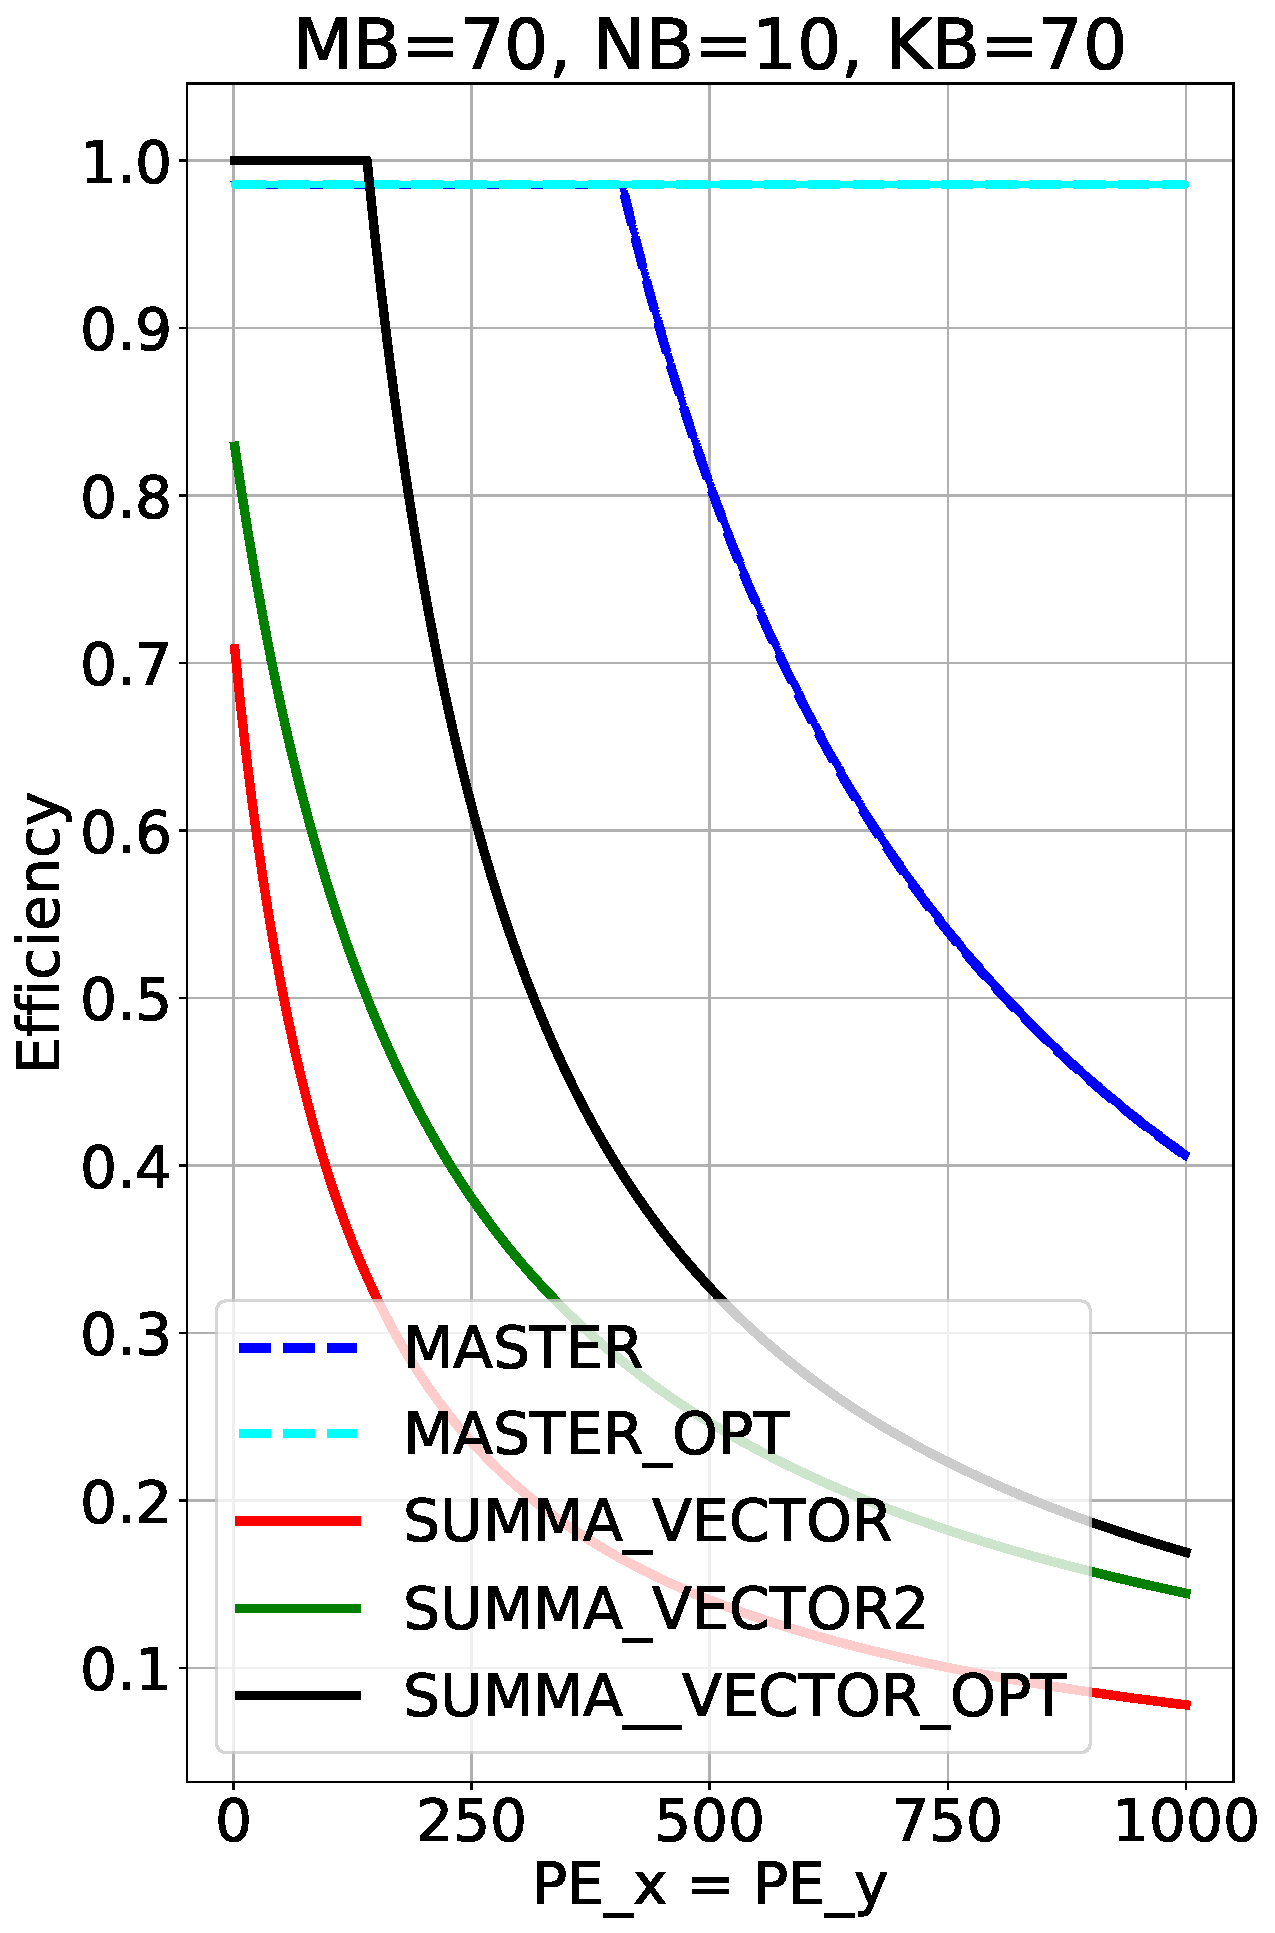
\includegraphics[width=\linewidth]{figures/efficiency_cost_70_10_70.pdf}
    %\caption{Non-ring.}
    %\label{fig:gemm_master_2}
  \end{subfigure}
  \caption{Performance simulation. ``MASTER": Equation~\ref{eq:master}; ``MASTER\_OPT": Equation~\ref{eq:master_2}; ``SUMMA\_VECTOR'': Equation~\ref{eq:summa_1}; ``SUMMA\_VERTOR2'': Equation~\ref{eq:summa_2}; ``SUMMA\_VECTOR\_OPT'': Equation~\ref{eq:summa_3}.}
  \label{fig:gemm_perf_simulate}
\end{figure}

Next, Table~\ref{table:exp_result} details some experimental and theoretical performance results.
%
Most of these experiments come from \texttt{test\_perf} in test\_matmul.
%
``Exp'' shorts for experimental, and ``Theo'' shorts for theoretical.
%
Numbers in bold are scenarios that \summa is better than \master.
%
From this table, we can see that 
\begin{itemize}
  \item the theoretical bound of \master possibly is between Equation~\ref{eq:master} and Equation~\ref{eq:master_2};
  \item the theoretical bound of \summa without optimization possibly is between Equation~\ref{eq:summa_1} and Equation~\ref{eq:summa_2};
  \item these results roughly follow the trends of their theoretical bounds.
\end{itemize}



\begin{table}[t!]
\caption{Performance results.}
%\footnotesize
\label{table:exp_result}
\centering
\begin{tabular}{cccc|ccc|cccc}
\toprule
\bf \makecell{K\\(hin)} & \bf \makecell{N\\(hout)} & \bf \makecell{M\\(batch)} & \bf \makecell{PE\_x\\(PE\_y)} & \bf \makecell{Exp\\ \master\\(cycles)} & \makecell{\bf Exp\\ \summa\\(cycles)} & \bf \makecell{Exp Ratio\\ \master/\summa} & \bf \makecell{Theo Eq\ref{eq:master}\\ \master\\ (cycles)}  & \bf \makecell{Theo Eq\ref{eq:master_2}\\ \master\\ (cycles)} & \bf \makecell{Theo Eq\ref{eq:summa_1}\\ \summa \\(cycles)} & \bf \makecell{Theo Eq\ref{eq:summa_2}\\ \summa \\(cycles)} \\
\midrule
128 & 128 & 128 & 16 & 5859 & 6946 & 0.84 & 6656 & 2352 & 7168 & 4608 \\
256 & 128 & 128 & 16 & 8874 & 13762 & 0.64 & 6656 & 4400 & 14336 & 9216 \\
128 & 256 & 128 & 16 & 11430 & 8996 & \bf 1.27 & 13312 & 4656 & 9216 & 7168 \\ 
256 & 256 & 128 & 16 & 17535 & 17863 & 0.98 & 13312 & 8752 & 18432 & 14336 \\
128 & 128 & 256 & 16 & 8002 & 10365 & 0.77 & 6912 & 4656 & 10240 & 7168 \\
256 & 128 & 256 & 16 & 12116 & 20626 & 0.58 & 8704 & 8752 & 20480 & 14336 \\
128 & 256 & 256 & 16 & 15803 & 14470 & \bf 1.09 & 13824 & 9264 & 14336 & 11264 \\
256 & 256 & 256 & 16 & 23982 & 28816 & 0.83 & 17408 & 17456 & 28672 & 22528 \\
128 & 128 & 384 & 16 & 10830 & 13875 & 0.78 & 7168 & 6960 & 13312 & 9728 \\
256 & 128 & 384 & 16 & 16969 & 27636 & 0.61 & 13056 & 13104 & 26624 & 19456 \\
128 & 256 & 384 & 16 & 21469 & 20022 & \bf 1.07 & 15872 & 13872 & 19456 & 15872 \\ 
256 & 256 & 384 & 16 & 33729 & 39924 & 0.84 & 26112 & 26160 & 38912 & 31744 \\
%10 & 10 & 10 & 10 & 348 & 293 & 1.18 & 325 & 212 & 107 \\
40 & 40 & 40 & 10 & 1289 & 1215 & \bf 1.06 & 1320 & 230 & 1120 & 640 \\ 
80 & 80 & 80 & 10 & 3636 & 3848 & 0.94 & 2720 & 1470 & 3520 & 2400 \\ 
720 & 20 & 720 & 10 & 27517 & 114820 & 0.23 & 26280 & 26310 & 92160 & 59040 \\
20 & 720 & 720 & 10 & 79132 & 28500 & \bf 2.77 & 38880 & 38910 & 27760 & 26840 \\ 

%\midrule
%Total & ${\frac{1}{3}} \times n^3$ & $$\\
%Total & & $O(N^2 \rank)$\\
\bottomrule
\end{tabular}
\end{table}


%\includegraphics{summa_gemm.gif}

%%%%%%%%%%%%%%%%%%%%%%%%%%%%%%%%%%%%%%%%%%%%%%%%%%%%%%%%%%%%%%%%%%%%%%%%%%
\section{MatMul in Machine Learning}
\label{sec:ml}
%\input{ml.tex}
%%%%%%%%%%%%%%%%%%%%%%%%%%%%%%%%%%%%%%%%%%%%%%%%%%%%%%%%%%%%%%%%%%%%%%%%%%
\section{Possible Optimizations towards \summa}
\label{sec:opt}
%!TEX root = matmul_wse.tex

\subsection{Block instead of Vector}

If using block instead of vector, then the number of iteration is $PE_x$ instead of $K$.
%
Therefore, if still considering the top right corner PE and FP16, in each iteration, the number cycles of FMAC is: $MB * NB * KB / 4$; while it needs $PE_x+MB \times KB/4$ cycles to receive $A$ (activation) and $PE_y+NB \times KB/2$ cycles to receive $B$ (weight).


In this case, Equation~\ref{eq:summa_1} becomes:
\begin{equation}
  MB \times NB \times KB/(MB \times NB \times KB +4 \times PE_x + 2 \times MB \times KB+4 \times PE_y + 2 \times NB \times KB)
  \label{eq:summa_4}
\end{equation}
%
Equation~\ref{eq:summa_2} becomes:
\begin{equation}
  MB \times NB \times KB/(MB \times NB \times KB +max(4 \times PE_x + 2 \times MB \times KB, 4 \times PE_y + 2 \times NB \times KB))
  \label{eq:summa_5}
\end{equation}
%
Equation~\ref{eq:summa_3} becomes:
\begin{equation}
  MB \times NB \times KB/max(MB \times NB \times KB, 4 \times PE_x + 2 \times MB \times KB, 4 \times PE_y + 2 \times NB \times KB)
  \label{eq:summa_6}
\end{equation}

This way relaxes the urgency of the communication and creates more rooms to overlap communication and computation, and Fig.~\ref{fig:gemm_perf_simulate_block} updates Fig.~\ref{fig:gemm_perf_simulate} with this optimization, which is called ``BLOCK'' instead of ``VECTOR''.


\begin{figure}[t!]
  \centering
  \begin{subfigure}{0.32\columnwidth}
    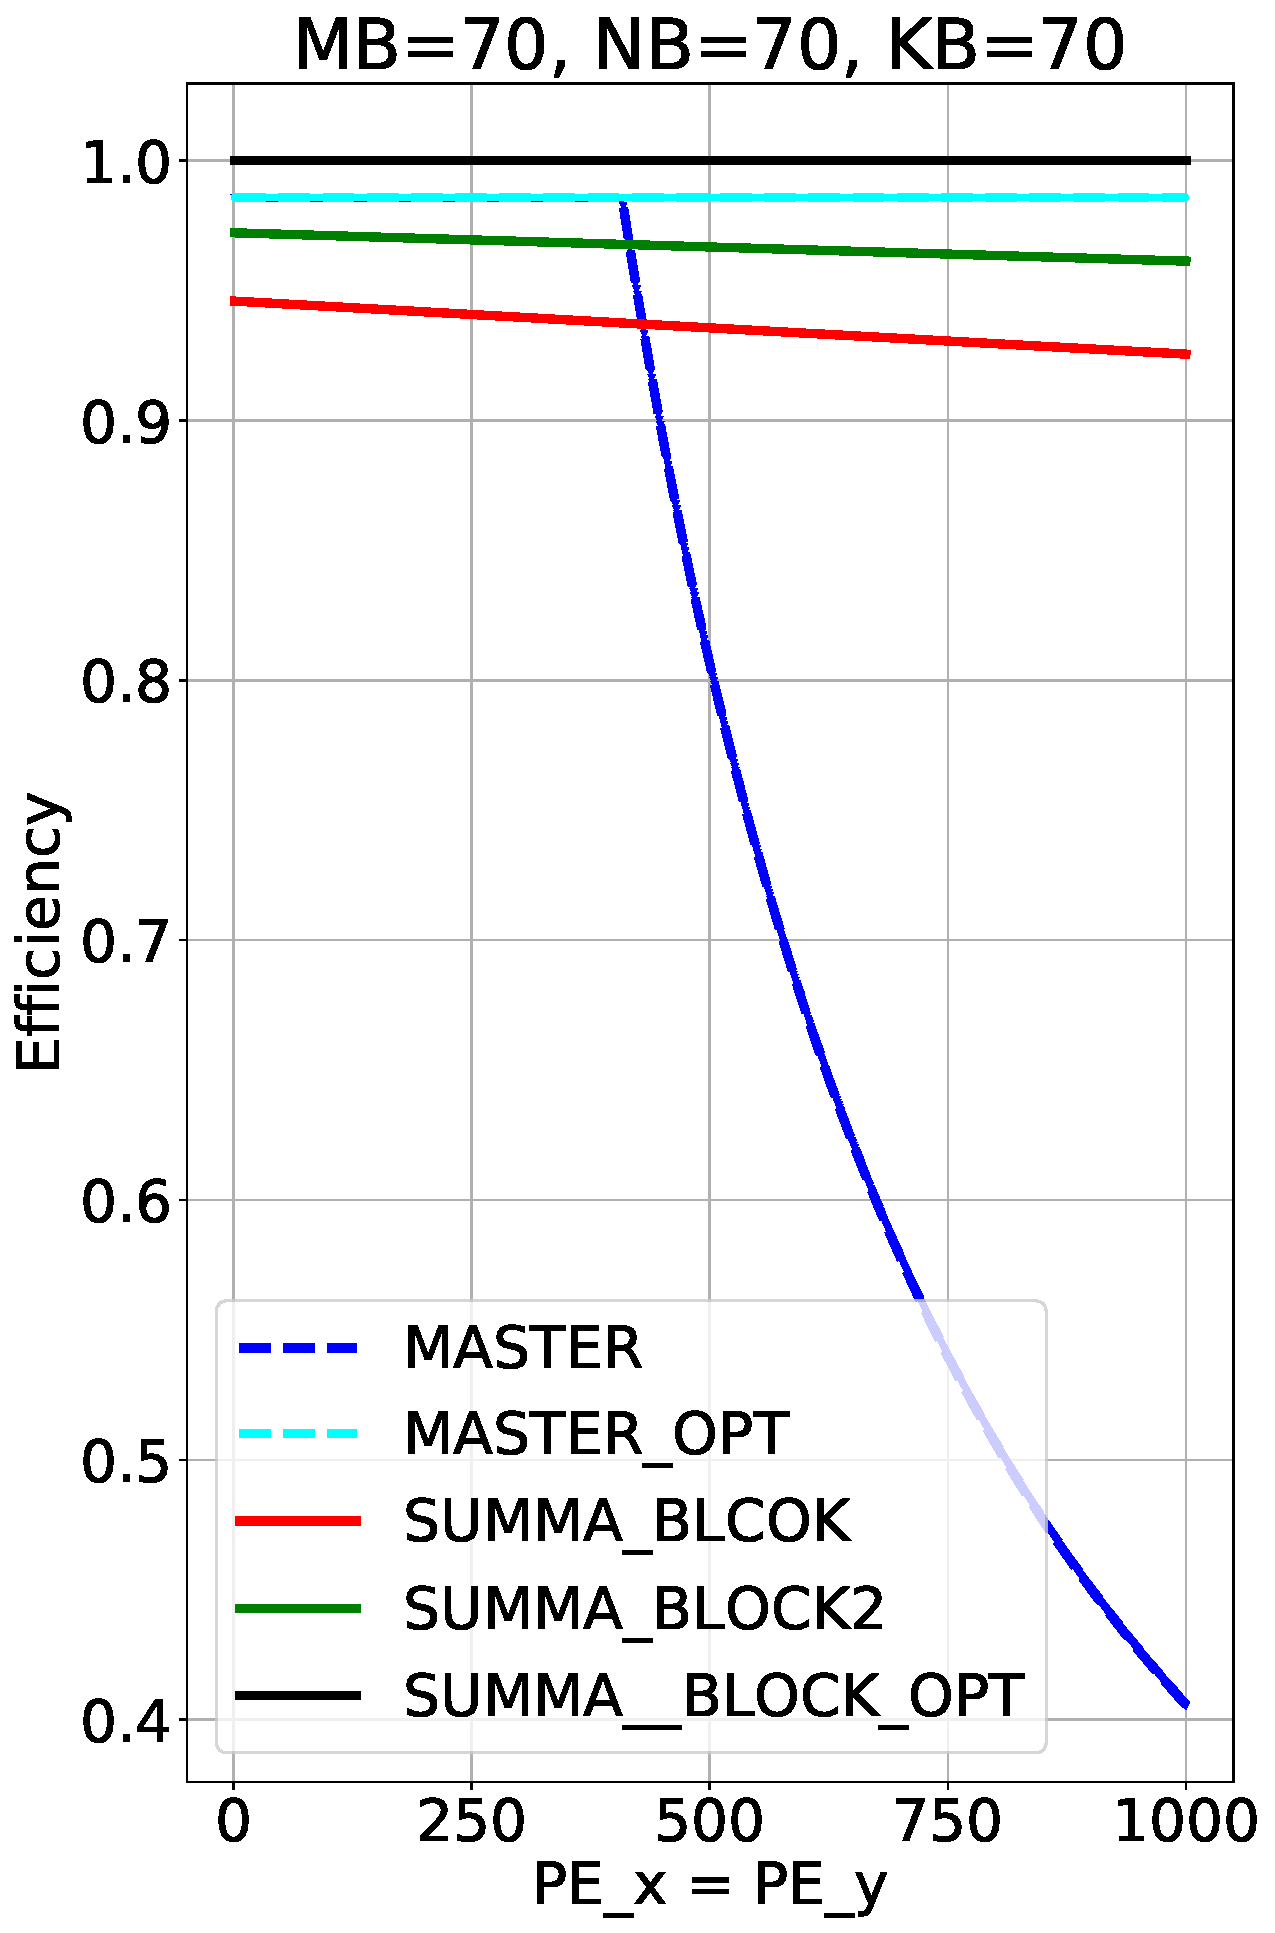
\includegraphics[width=\linewidth]{figures/efficiency_cost_block_70_70_70.pdf}
    %\caption{.}
    %\label{fig:gemm_master_1}
  \end{subfigure}
  \hfill
  %
  \begin{subfigure}{0.32\columnwidth}
    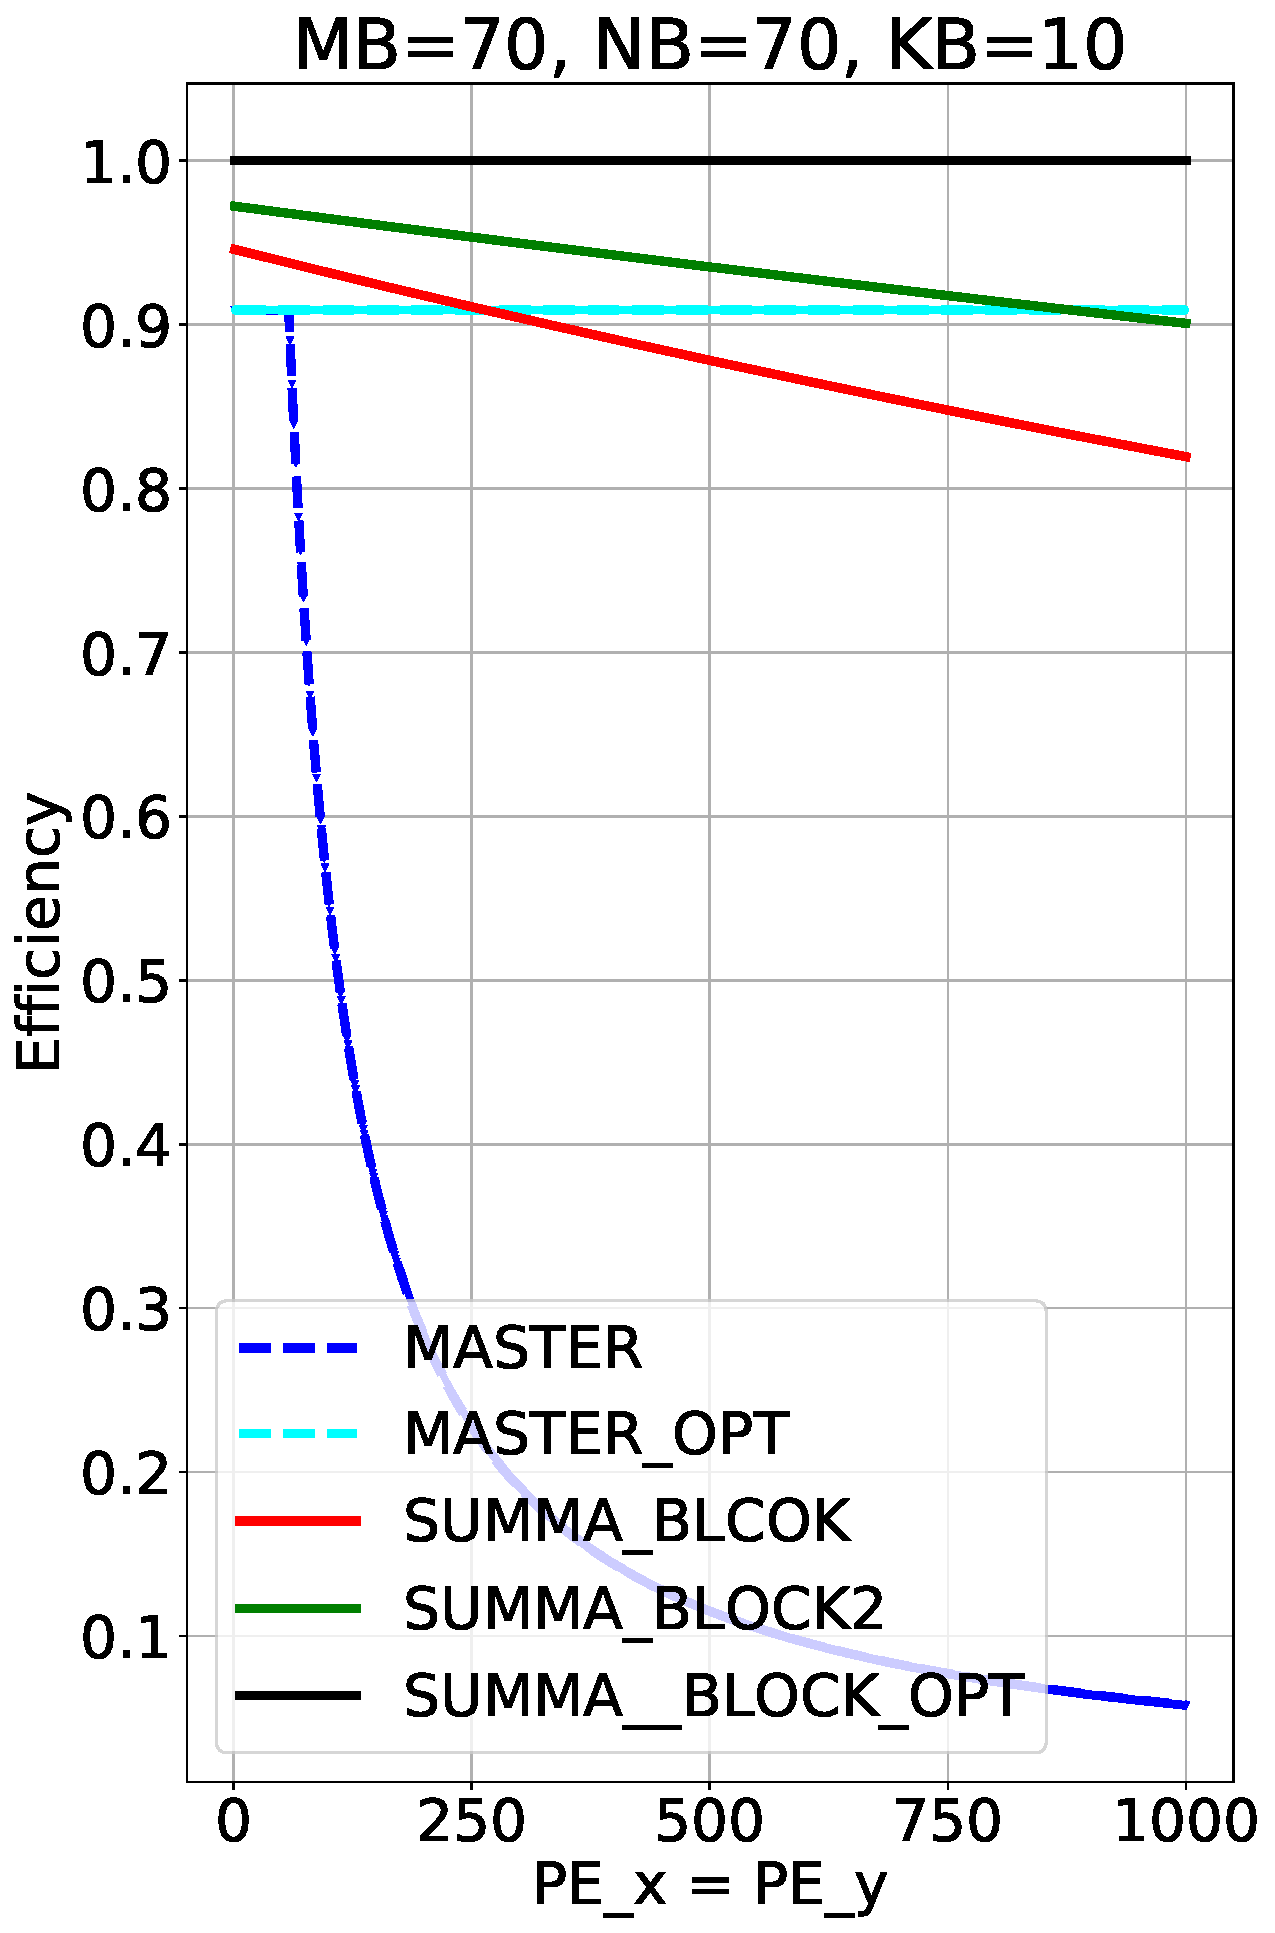
\includegraphics[width=\linewidth]{figures/efficiency_cost_block_70_70_10.pdf}
    %\caption{Non-ring.}
    %\label{fig:gemm_master_2}
  \end{subfigure}
  \hfill
  %
  \begin{subfigure}{0.32\columnwidth}
    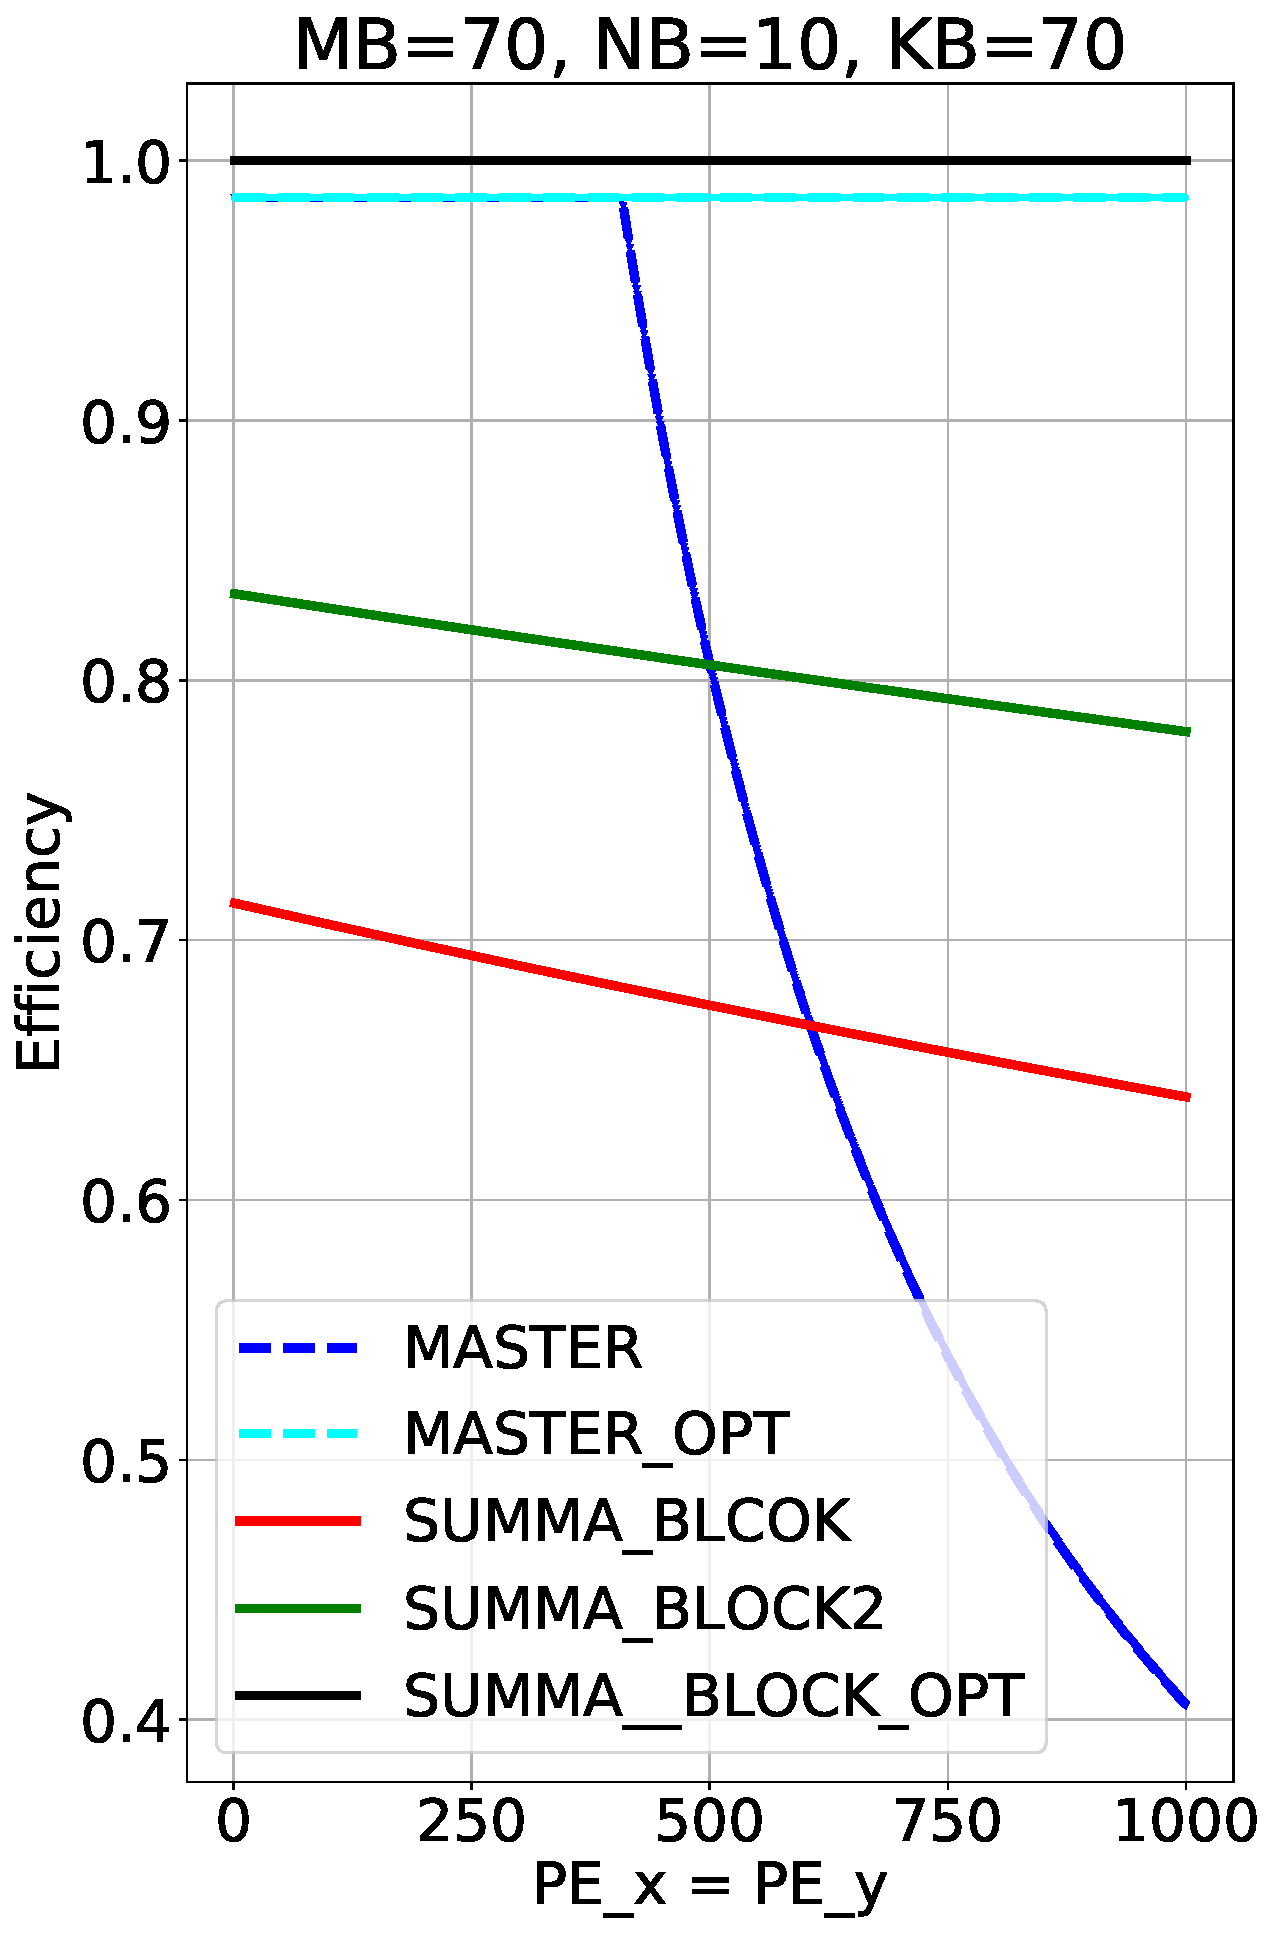
\includegraphics[width=\linewidth]{figures/efficiency_cost_block_70_10_70.pdf}
    %\caption{Non-ring.}
    %\label{fig:gemm_master_2}
  \end{subfigure}
  \caption{Performance simulation. ``MASTER": Equation~\ref{eq:master}; ``MASTER\_OPT": Equation~\ref{eq:master_2}; ``SUMMA\_BLOCK'': Equation~\ref{eq:summa_4}; ``SUMMA\_BLOCK2'': Equation~\ref{eq:summa_5}; ``SUMMA\_BLOCK\_OPT'': Equation~\ref{eq:summa_6}.}
  \label{fig:gemm_perf_simulate_block}
\end{figure}
 

%\subsection{Overlap Computation and Communication?}


%\subsection{FIFO??}


\subsection{Ideal}


The ideal \summa should be (1) communication perfectly by computation (2) pipelined.
%
Therefore, the total number of cycles for a MatMul problem on FP16 is $max(MB \times NB \times K / 4, PE_x + MB \times K/2,  PE_y + NB \times K/2)$:
Equation~\ref{eq:summa_3} becomes:
\begin{equation}
  MB \times NB \times K/max(MB \times NB \times K, 4 \times PE_x + 2 \times MB \times K, 4 \times PE_y + 2 \times NB \times K)
  \label{eq:summa_7}
\end{equation}
%
Fig.~\ref{fig:gemm_perf_simulate_ideal} mimics three scenarios of square matrices with relative small sizes.
%
{\bf However, this is the ideal, and I'm not sure whether it's achievable or not.}


\begin{figure}[t!]
  \centering
  \begin{subfigure}{0.32\columnwidth}
    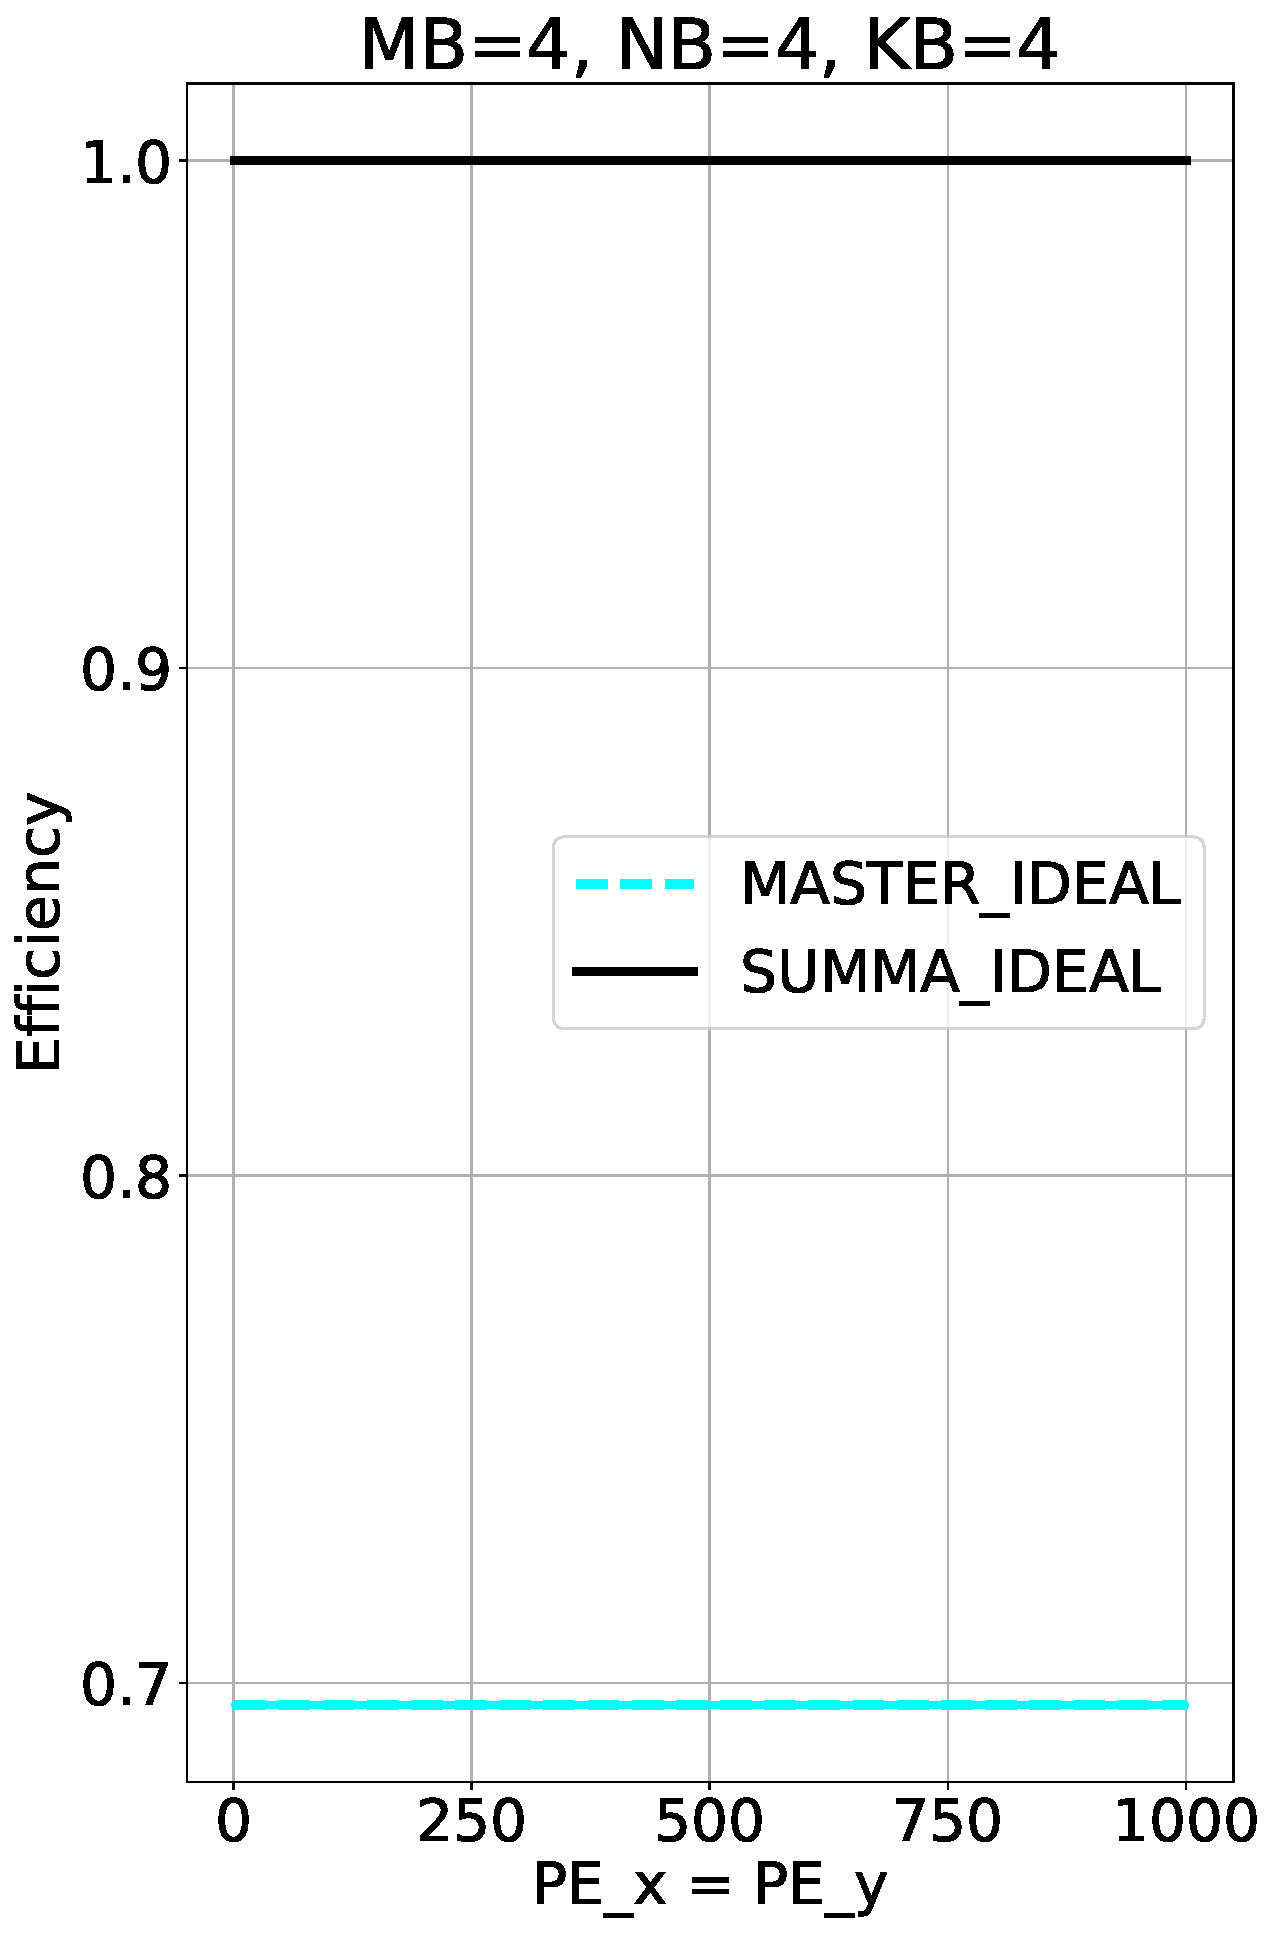
\includegraphics[width=\linewidth]{figures/efficiency_cost_ideal_4_4_4.pdf}
    %\caption{.}
    %\label{fig:gemm_master_1}
  \end{subfigure}
  \hfill
  %
  \begin{subfigure}{0.32\columnwidth}
    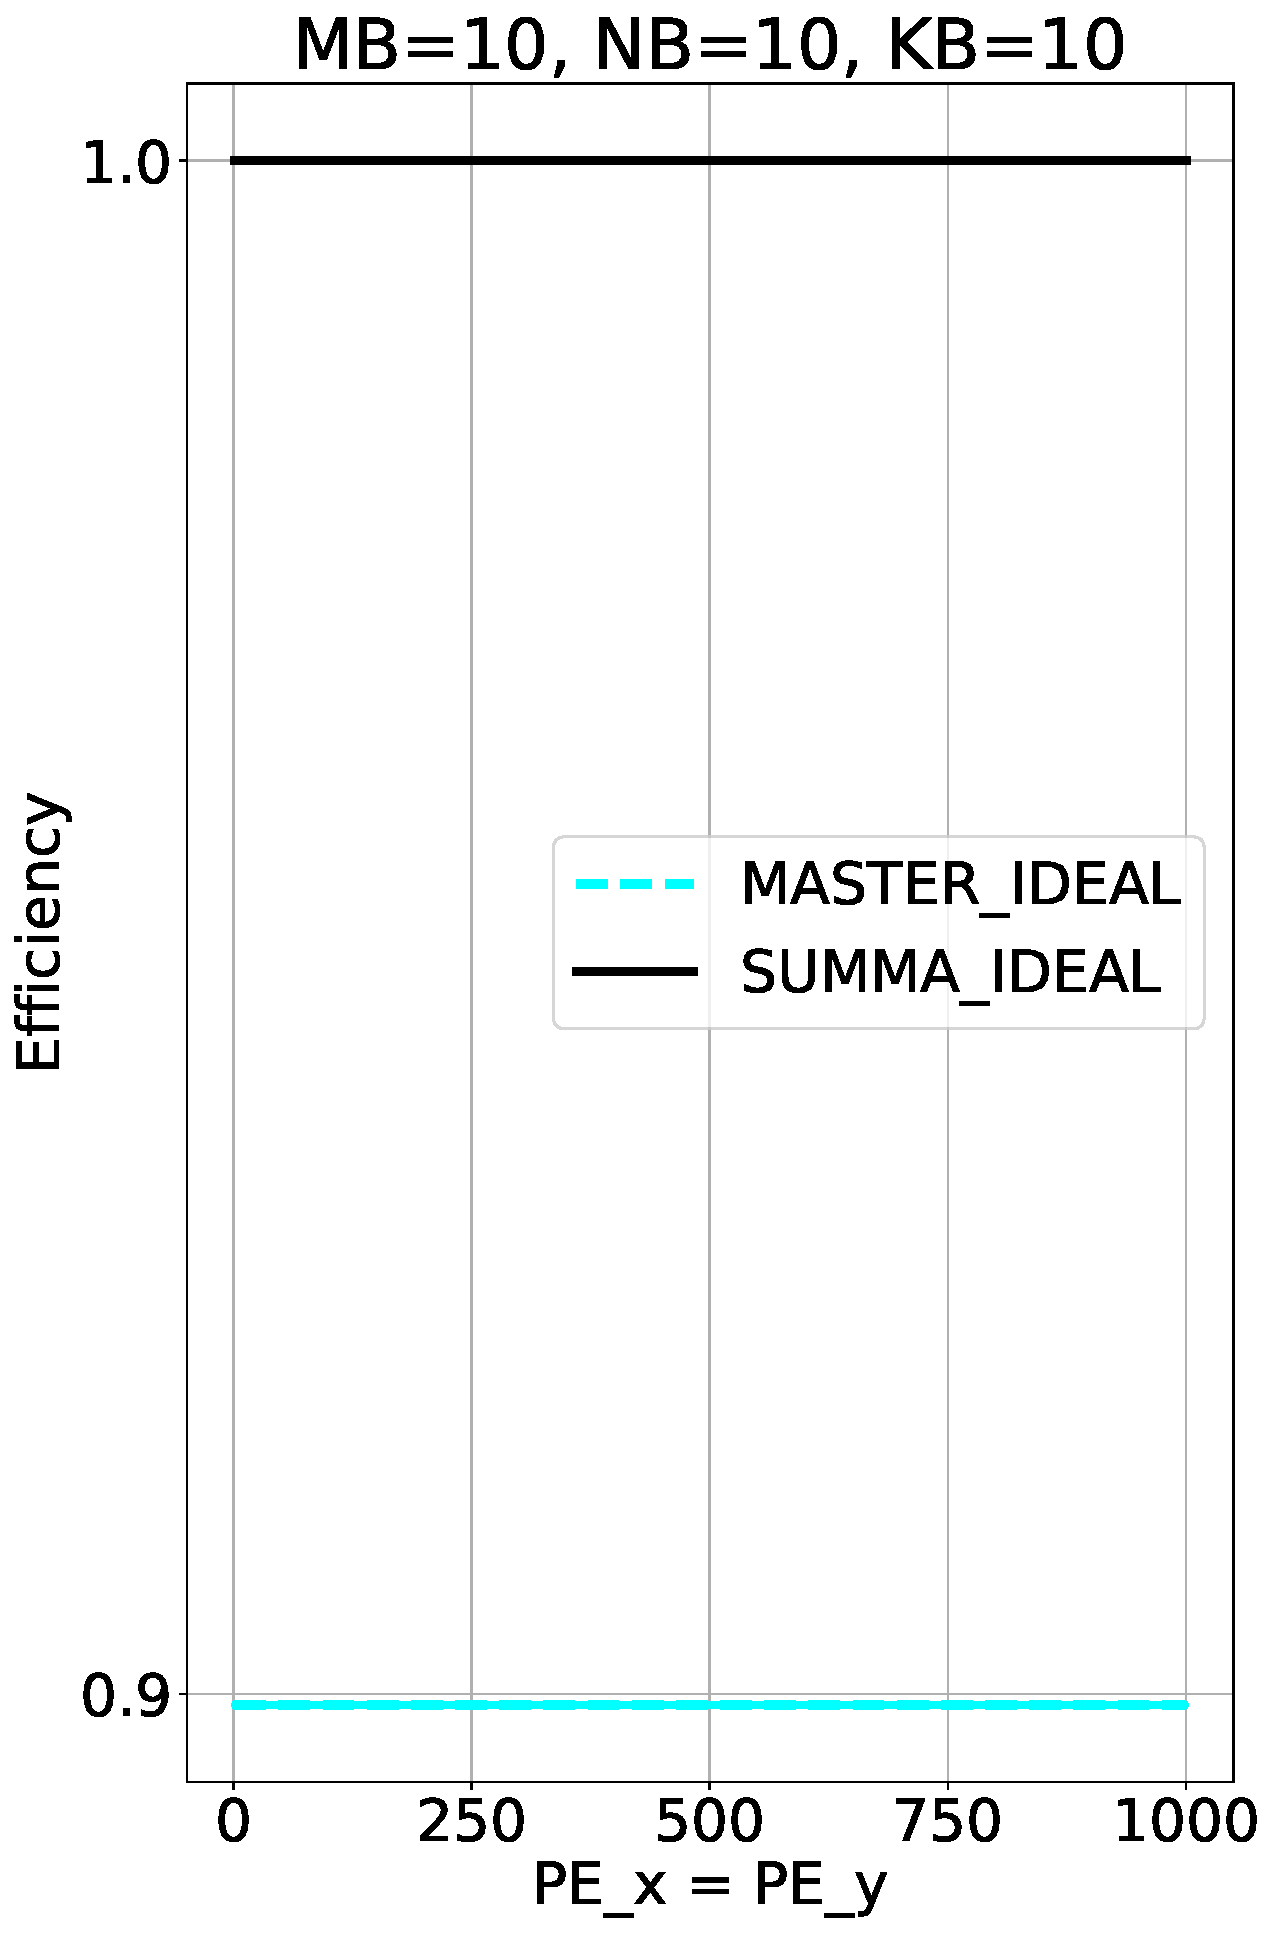
\includegraphics[width=\linewidth]{figures/efficiency_cost_ideal_10_10_10.pdf}
    %\caption{Non-ring.}
    %\label{fig:gemm_master_2}
  \end{subfigure}
  \hfill
  %
  \begin{subfigure}{0.32\columnwidth}
    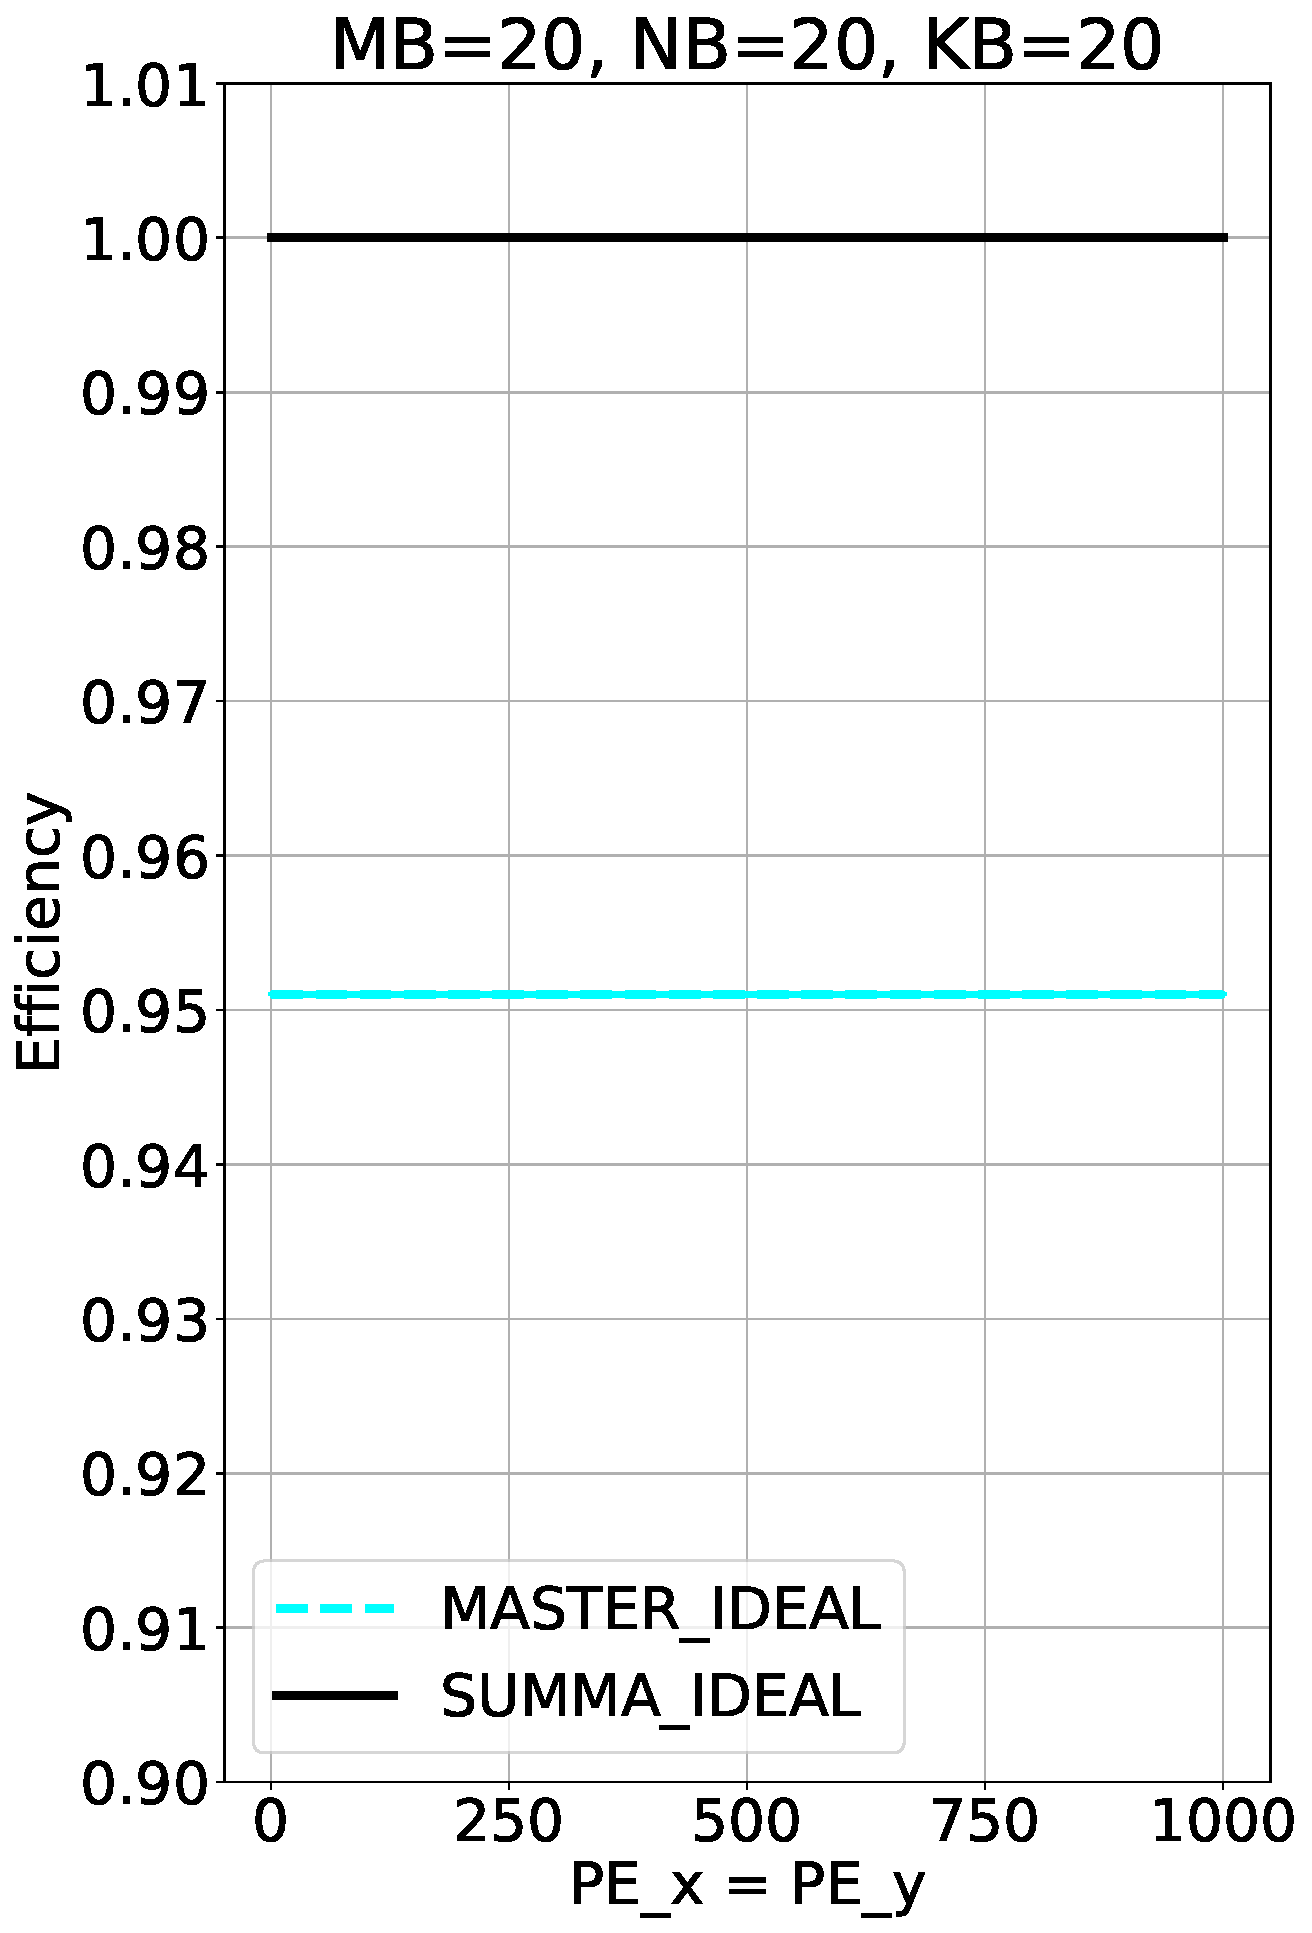
\includegraphics[width=\linewidth]{figures/efficiency_cost_ideal_20_20_20.pdf}
    %\caption{Non-ring.}
    %\label{fig:gemm_master_2}
  \end{subfigure}
  \caption{Performance simulation. ``MASTER\_IDEAL": Equation~\ref{eq:master_2}; ``SUMMA\_IDEAL'': Equation~\ref{eq:summa_7}.}
  \label{fig:gemm_perf_simulate_ideal}
\end{figure}





%%%%%%%%%%%%%%%%%%%%%%%%%%%%%%%%%%%%%%%%%%%%%%%%%%%%%%%%%%%%%%%%%%%%%%%%%
\section{Summary}
%\textbf{Acknowledgments.}
%\input{ack.tex}
%%%%%%%%%%%%%%%%%%%%%%%%%%%%%%%%%%%%%%%%%%%%%%%%%%%%%%%%%%%%%%%%%%%%%%%%%%
% The next two lines define the bibliography style to be used, and the bibliography file.

% trigger a \newpage just before the given reference
% number - used to balance the columns on the last page
% adjust value as needed - may need to be readjusted if
% the document is modified later
\IEEEtriggeratref{18}

\bibliographystyle{IEEEtran}
\bibliography{ref}

\begin{comment}
% If your work has an appendix, this is the place to put it.
\appendix
\newpage
\section{XXXXXX}
\label{sec:appendix_tilesize}

\end{comment}



%\clearpage
%\listoftodos[Notes]

\end{document}
